\chapter[Explicit predictive current control]{Explicit model predictive control of a current source buck-type rectifier}\label{BASIC:sec:MPC_CSR}

\section{Literature overview}

%============ USAGE OF CURRENT SOURCE RECTIFIERS
Current source rectifiers (CSR) are widely used in frond-end power electronic converter for the uncontrollable or controllable DC-bus in industrial and commercial applications. They have maintained their position through many applications, with uses such as medium-voltage high-power drives \cite{vajda2017limiting}, \cite{ghalem2010six} STATCOMs \cite{gupta2014two} and renewable systems \cite{chen2016single}, \cite{exposto2015predictive}. They have a plain and reliable circuit structure, which makes them attractive for simple control design. The CSRs are traditionally controlled by state feedback, or classic cascaded linear control loops such as PI controllers. These simple control applications are suitable for induction motor control \cite{chebre2011speed}, and other electromechanical actuators \cite{salloum2014robust}, and unusual topologies \cite{neukirchner2017voltage}. Also, worth mentioning of self-tuning variants of PI controllers \cite{tahri2012digital}.\\
%============ MODULATION OF CSR
 In the past, the modulation methods used were trapezoidal pulse width modulation techniques (TPWM), or application of pulse patterns calculated off-line for selective harmonic elimination (SHE). More recently, current space vector modulation (SVM) has been used for the synthesis of the transistor control signals \cite{gao2017model}. Even so, AC-side harmonic elimination could still be an issue at lower switching frequencies where LCL filtering (inductive-capacitive-inductive) would be advised \cite{han2010control}.\\
%============ TOPOLOGIES OF CSR
In order to keep switching frequencies low and to minimize switching losses, new topologies and hybrid modulations are used, mixing TPWM and SHE depending on the grid frequency \cite{venkatraman2018multilevel}.\\
%============ BENEFITS OF CSR
    In terms of the amplitude of the grid and DC-link voltages, CSRs exhibit a step-down conversion. When used as DC voltage source, the rectifier can output a lower DC voltage without the need of a grid-side transformer, as is usually employed in voltage source rectifiers (VSR). Because of their current source behavior, CSRs can easily be paralleled and provide inherent short-circuit protection, representing an excellent potential in DC power supply applications \cite{feroura2017finite}, \cite{yan2015study}.\\		
%============ GENERAL POWER ELECTRIC CONTROL
    There are several control strategies in addition to classical PI control for applications in this domain. Self-adapting control methods are on the rise with more sophisticated algorithms in the field of fuzzy logic \cite{urmos2017application}. They are capable of handling increasingly more complicated models and systems with high dynamics and accuracy \cite{chatterjee2008augmented}, \cite{haidegger2012simulation}, and even without establishing and validating classical state-space models \cite{vrkalovic2018model}. The other filed is the sliding mode control, which can achieve good dynamic performance and handle non-linearity. Still, they might also introduce chattering, which can be very undesirable when applied to real-life systems like in \cite{regaya2014new} and \cite{szell2014mathematical}. Additionally in \cite{ahmed2014model} the validity of an MPC-based, digital pulse width modulation control strategy for single-phase voltage source rectifiers is discussed, further confirming the validity of this method in control systems.\\	
%============ PREDICTIVE POWER ELECTRIC CONTROL		
    In the linear domain implicit model predictive control (IMPC or MPC) is a fair solution due its effectiveness in power electronics because of its configurable cost function and such scalable nature \cite{kelemen2010constrained}, \cite{ahmed2014model}. In this field also finite-state solutions are present which can be considered also predictive control, where the modulation scheme’s defined states serve as optimization potential \cite{rivera2013predictive}, \cite{godlewska2015predictive}. As a further step adaptive application was established to tackle parameter estimation problems for better performance \cite{muthukumar2016adaptive}\\	
%============ EXPLICIT PREDICTIVE CONTROL
    Recently, beside implicit, finite-state, and adaptive predictive control, explicit model predictive control has emerged in the field of power electronics \cite{kutasi2010constrained}. Establishing the MPC cost function can range widely depending on the expected dynamics, degree of noise cancellation, and model complexity. Additionally, the current limitation can also be implemented introducing constraints in the modulation algorithm.\\	

\section{Three-phase buck-type rectifiers}\label{BASICCSR:sec:CSR}

Three-phase controlled rectifiers have a wide range of applications, from small rectifiers to large high-voltage direct-current transmission systems. They are used e.g. at electrochemical processes, many kinds of motor drives, traction equipment, controlled power supplies. In this thesis only force commuted rectifiers are examined, which are built with semiconductors (IGBTs in this case) with gate-turn-off capability. The gate-turn-off capability allows full control of the converter, because valves can be switched ON and OFF whenever is required. This allows the commutation of the valves, hundreds of times in one period that is not possible with line-commutated rectifiers, where IGBTs are switched ON and OFF only once a cycle. This has the following advantages:

\begin{itemize}
\item The current or voltage can be (pulse width) modulated, generating less harmonic contamination.
\item The power factor (ratio of the real and reactive power) can be controlled and even it can be made leading, signifies that the load is capacitive, as the load “supplies” reactive power.
\item They can be built as voltage-source or current-source based on the required application.
\item The reversal of power in switching rectifiers is by reversal of voltage at the DC link. This allows force commutated rectifiers can be implemented for both, reversal of voltage or reversal of current.
\end{itemize}

There are two ways to implement force commutated three phase rectifiers, as a current-source rectifier (Fig.\ref{BASICMPC:fig:CSR}), where power reversal is by DC voltage reversal, and as a voltage-source rectifier (Fig.\ref{BASICMPC:fig:VSR}), where power reversal is is solved by current reversal at the DC link.


\begin{figure}[h]
                \centering
                \begin{subfigure}[b]{0.9\textwidth}
                    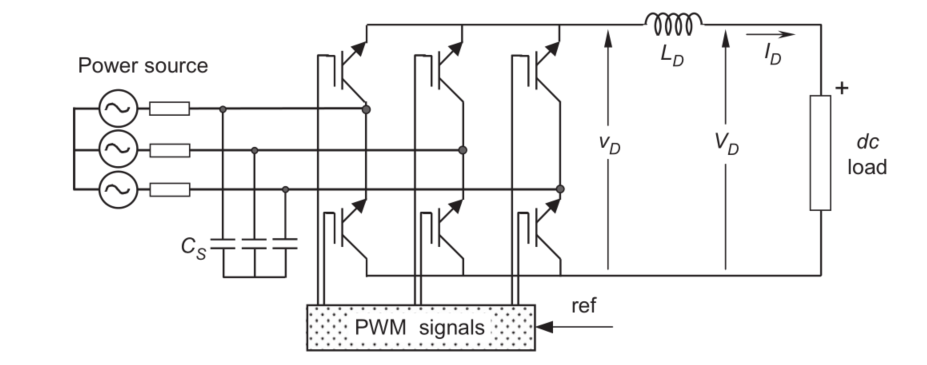
\includegraphics[width=\textwidth]{EMPC_PNG_Pics/BasicCurrentRectifiers.png}
                    \caption{\centering Current source rectifier with capacitive filtering and choke inductance.}
                    \label{BASICMPC:fig:CSR}
                \end{subfigure}
                ~ %add desired spacing between images, e. g. ~, \quad, \qquad, \hfill etc.
                  %(or a blank line to force the subfigure onto a new line)
                \begin{subfigure}[b]{0.9\textwidth}
                    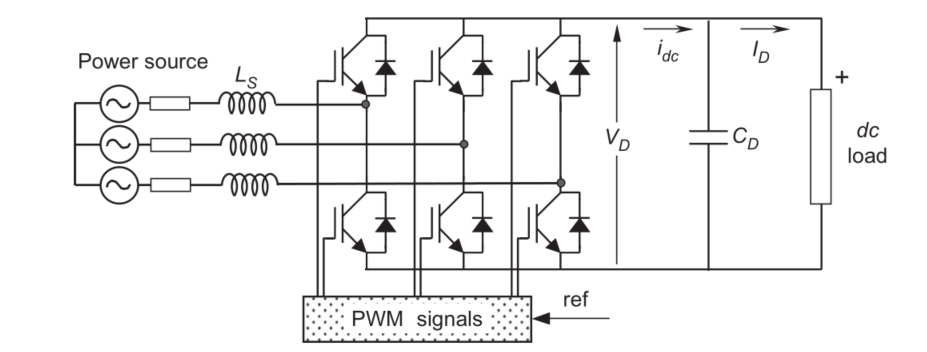
\includegraphics[width=\textwidth]{EMPC_PNG_Pics/BasicVoltageRectifiers.png}
                    \caption{\centering Voltage source rectifier with inductive filtering and DC voltage smoothing capacitance.}
                    \label{BASICMPC:fig:VSR}
                \end{subfigure}
                 %add desired spacing between images, e. g. ~, \quad, \qquad, \hfill etc.
                %(or a blank line to force the subfigure onto a new line)
                %\begin{subfigure}[b]{0.48\textwidth}
                    %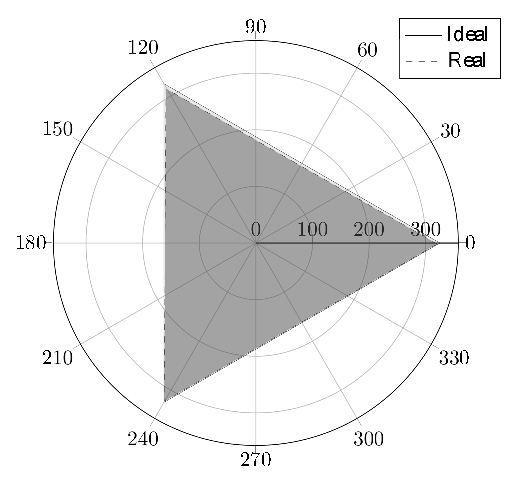
\includegraphics[width=\textwidth]{Unblance_EPS_Pics/EPS_images/square.eps}
                    %\caption{Low correlation with opposed amplitude deviation. The norm values are $G=9322$ and $TDV=0.5198$.}
                    %\label{fig:cases_C}
                %\end{subfigure}
                %~
                %\begin{subfigure}[b]{0.48\textwidth}
                    %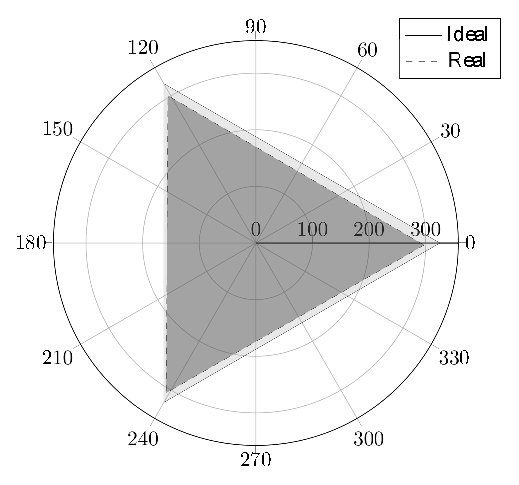
\includegraphics[width=\textwidth]{Unblance_EPS_Pics/EPS_images/circle.eps}
                    %\caption{\centering Low correlation with uniform voltage drop. The norm values are $G=6280$ and $TDV=0.156$.}
                    %\label{fig:cases_D}
                %\end{subfigure}


                \caption{Basic topologies of force commuted rectifiers.}
            \end{figure}

%\begin{figure}[!ht]
        %\centering
        %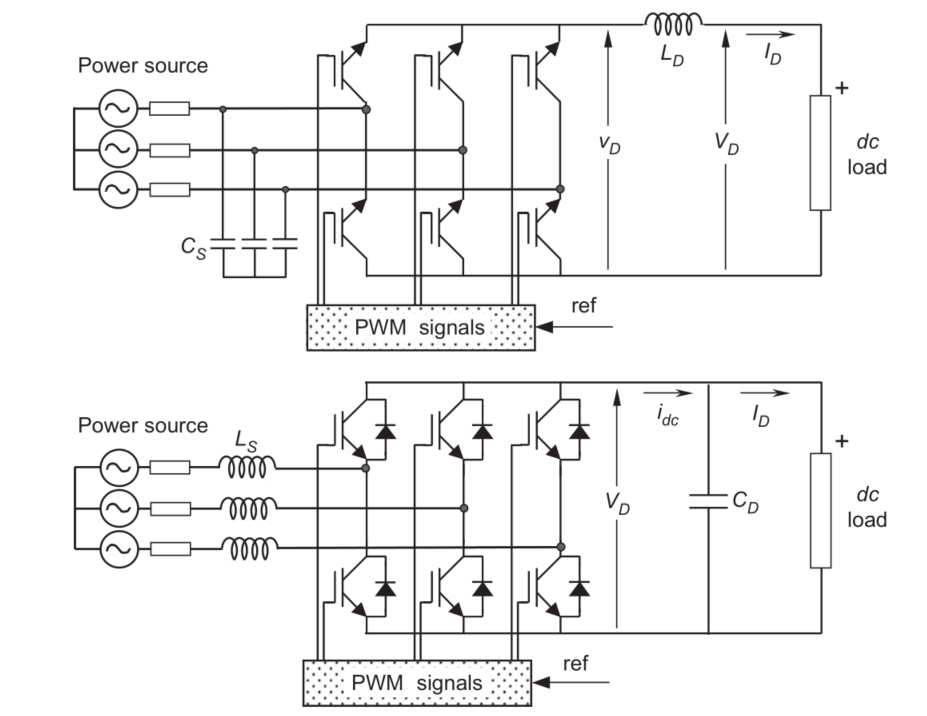
\includegraphics[width=0.9\textwidth]{EMPC_PNG_Pics/CurrentVoltageRectifiers.png}
        %\caption{Basic topologies of force commuted rectifiers.}
        %\label{BASICCSR:fig:topologies}
    %\end{figure}


As  general case be a front-end  converter power supply (e.g. lighting or telecommunications) shall be designed such that it should have approximately these general characteristics: sinusoidal main currents, unity power factor, high power density and simplicity of the power circuit structure. Two structures are most fitted for the task. First a boost-type input rectifier (e.g., Vienna rectifier, \cite{kolar1996design}), that typically features two $400$ V output voltages with a three-level isolated  DC-DC  converter  or  two  isolated  DC-DC  output  stage (see Fig. \ref{EMPC:fig:network} in Ch.5.). The second candidate is the buck-type  input  rectifier (or current source rectifier (CSR))  (conventionally  six-switch topologies as proposed in \cite{zargari1993current}, \cite{sato1993state}) with only one two-level isolated  DC-DC  converter  output  stage.  Also the  input  stage  can be realized as a three-switch topology with considerably  lower  system  complexity  as  compared  to  the boost-type structure. In particular, the number of utilized active and passive components is much lower. Furthermore, there is no middle-point that has to be stabilized, as this is the case for the boost-type structures, making control and active filter design less complex. Further system advantages are the potential of direct start-up and the implicit over current protection in case of an output short circuit. Therefore, these topologies of high interest for many safety critical applications as such future electric aircraft, or automotive applications or as power supplies for process technology \cite{nussbaumer2007comprehensive}.
The three-switch buck rectifier topology was first proposed in \cite{malesani1987three}. In \cite{itoh1989steady} and \cite{tooth2000effects}, aspects of the system modulation and control have been treated. The application of the topology used as an active filter is discussed in \cite{salo2005three}.  The addition of a DC-DC output boost-stage has been proposed in \cite{baumannnew} in order to maintain 400 V output voltage for a wide input voltage range and for the case of unbalanced mains as, e.g., the loss of one phase.

\myparagraph{Basic operation principles}\label{BASICCSR:sec:OperationPrinciple}

For the derivation of the relative on-times of the three buck transistors $S_i$ with the following assumptions are made for clarity and facilitation of calculations:
\begin{itemize}
	\item The AC-side filter capacitor voltages ($v_{c_p}$, where $p\in\{1,2,3\}$) at the input of the CSR are sinusoidal and in phase with the main harmonic component of voltage.
	
	\begin{equation}
        \begin{array}{rcl}
            v_{c_1}&=&\widehat{v}_c\cos(\omega t)\\
						v_{c_2}&=&\widehat{v}_c\cos(\omega t-2\pi/3)\\
						v_{c_3}&=&\widehat{v}_c\cos(\omega t+2\pi/3),\\
        \end{array}
        \label{BASICMPC:equ:phasorvect}
    \end{equation}
	where $\omega$ is the network voltage's angular velocity.
	
	\item The mains currents are assumed to be equal to the fundamental component of the rectifier input currents.
	\item The current in the DC output inductor $L_{D}$ is not affected by the high frequency ripple due to the switching operation.
\end{itemize}

 For achieving ohmic mains behavior also in case of unbalanced fundamental harmonics conditions the explained modulation method can still be utilized, however, additionally the control structure presented in \cite{baumann2005novel} has to be employed.\\
The waveforms of the phase and line-to-line mains voltages are divided into twelve sectors of $\frac{\pi}{6}$ rad wide shown in Fig.\ref{BASICCSR:fig:waves}. The following calculations are based on the analysis of the first sector which is characterized by the voltage harmonic phase relation. For the remaining sectors the calculations can be accomplished in an similar manner \cite{nussbaumer2007comprehensive}.

\begin{figure}[!ht]
        \centering
        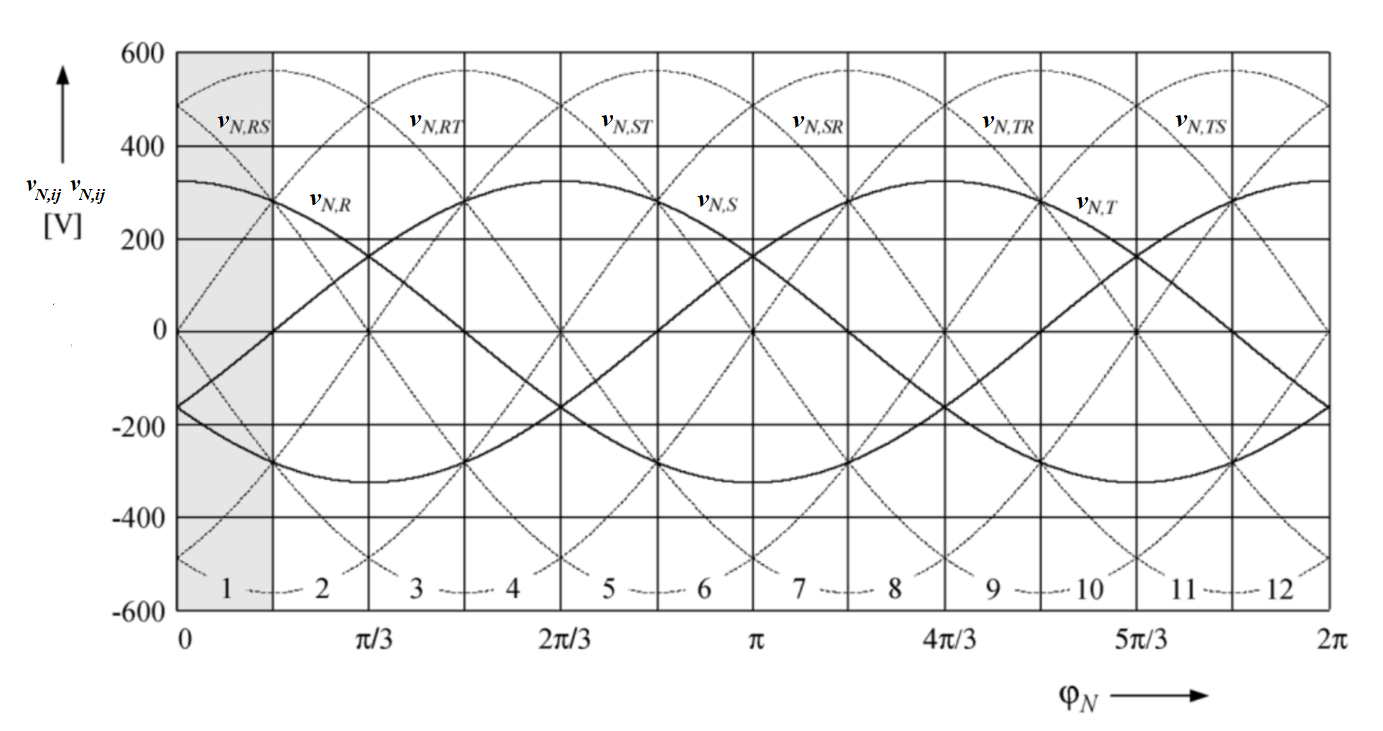
\includegraphics[width=\textwidth]{EMPC_PNG_Pics/Waves.png}
        \caption{Phase voltages $v_{i}$, where line-to-line voltages $v_{N,ij}=v_{N,i}-v_{N,j}$, $(i,j)\in\{R,S,T\}$ and sectors $1$ to $12$ being defined by the different relations of the instantaneous values of the mains phase voltages for $v = 400 V$}
        \label{BASICCSR:fig:waves}
    \end{figure}
		
		Accordingly, on AC side, if conditions are favorable, inductor current can appear in an instant of time either in two out
of three phases or in none. In this modulation technique, the switches in each converter leg can conduct only one at the time (aside from zero states, where both upper and lower switches are conducting). When the upper leg is conducting it is indicated by `$1$', when the lower  `$-1$' and when neither `$0$'. As such the choice whether upper or lower switch of the leg conducts current depends of the reference current vector's sector location.
According to the actual switch combination the DC link current shaped by the choke inductance, and distributed to two of the input phases or the freewheeling diode. With this, the input current space vectors can be calculated for each of the before-mentioned switching states. Generally the space vector of three-phase quantities (e.g., for the rectifier input current) are described as:

\begin{equation}
        \begin{array}{rcl}
            \vec{i}&=&\frac{2}{3}\left(\vec{i}_a+\vec{i}_be^{\frac{j\pi}{3}}+\vec{i}_bc^{\frac{4j\pi}{3}}\right).\\
        \end{array}
        \label{BASICCSR:eqn:currents_all}
    \end{equation}
		
		Based on \ref{BASICCSR:eqn:currents_all} the corresponding active space vectors in the first sector can be obtained as:
		
		\begin{equation}
        \begin{array}{rcl}
            \vec{i}_{(1,0,-1)}=\vec{i}_1&=&2i_{dc}e^{j\pi/6}/\sqrt{3}\\
						\vec{i}_{(0,1,-1)}=\vec{i}_2&=&2i_{dc}e^{j\pi/2}/\sqrt{3}\\
						\vec{i}_{(-1,1,0)}=\vec{i}_3&=&2i_{dc}e^{j5\pi/6}/\sqrt{3}\\
        \end{array}
        \label{BASICCSR:eqn:currents}
    \end{equation}
		
		The resulting discrete space vectors can be used to synthesize desired current
space vector $\vec{i}_{ref}$.

The modulation methods were evaluated in and chosen for this paper based on \cite{moussaoui2005open}, which ensures minimum switching-losses, minimum ripple values of the input capacitor voltages and of the output inductor current. According to this modulation, each pulse interval comprises two active states and a freewheeling state, arranged symmetrically about the middle of the pulse interval (see Table \ref{EMPC:tbl:sequence}). For more in depth functional description see section \ref{EMPC:sec:Modulation}.

\subsection{Coordinate transformations}

In section \ref{EMPC:sec:ModelofCSR} the three phase current source rectifier's (CSR) equations are converted to different coordinate spaces.

\subsubsection{Clarke transformation}\label{BASICCSR:sec:Clarke}

In electrical engineering, Clarke transformation is a mathematical transformation employed to simplify the analysis of three-phase circuits. Conceptually it is similar to the Park transformation. One very useful application is the generation of the reference signal used for space vector modulation control of three-phase inverters. The transformation follows:

\begin{equation}
        \begin{array}{rcl}
            \textbf{i}_{\alpha\beta\gamma}(t)&=&T_{Clarke}\textbf{i}_{abc}(t)
            \begin{bmatrix}
            1& -\frac{1}{2}& -\frac{1}{2}\\
            0& \frac{\sqrt{3}}{2}& -\frac{\sqrt{3}}{2}\\
            \frac{1}{2}& \frac{1}{2}& \frac{1}{2}\\
            \end{bmatrix}
            \begin{bmatrix}
            i_a(t)\\
            i_b(t)\\
            i_c(t)\\
            \end{bmatrix},
        \end{array}
        \label{BASICCSR:eqn:Clarke}
    \end{equation}

    where $\textbf{i}_{abc}$ is the generic three phase current sequence, and $\textbf{i}_{\alpha\beta\gamma}$ is given by the transformation.

    \subsubsection{Park transformation}\label{BASICCSR:sec:Park}

The Park transformation is a tensor that rotates the reference frame of a three-element vector or a three-by-three element matrix in an effort to simplify analysis. The transform can be used to rotate the reference frames of AC waveforms such that they become DC signals. Simplified calculations can then be carried out on these dc quantities before performing the inverse transform to recover the actual three-phase ac results. As an example, the Park transform is often used in order to simplify the analysis of three-phase synchronous machines or to simplify calculations for the control of three-phase inverters. In analysis of three-phase synchronous machines the transformation transfers three-phase stator and rotor quantities into a single rotating reference frame to eliminate the effect of time-varying inductances. The transformation follows:


\begin{equation}
        \begin{array}{rcl}
            \textbf{i}_{dq0}(t)&=&T_{Park}\textbf{i}_{abc}(t)
            \sqrt{\frac{2}{3}}\begin{bmatrix}
            \cos(\theta)& \cos(\theta-\frac{2\pi}{3})& \cos(\theta+\frac{2\pi}{3})\\
            -\sin(\theta)& -\sin(\theta-\frac{2\pi}{3})& -\sin(\theta+\frac{2\pi}{3})\\
            \frac{\sqrt{2}}{2}& \frac{\sqrt{2}}{2}& \frac{\sqrt{2}}{2}\\
            \end{bmatrix}
            \begin{bmatrix}
            i_a(t)\\
            i_b(t)\\
            i_c(t)\\
            \end{bmatrix},
        \end{array}
        \label{BASICCSR:eqn:Park}
    \end{equation}

    where $\theta$ is instantaneous angular position of an arbitrary frequency.

\section{Model based predictive control}

\subsection{Quadratic optimization and predictive control}\label{BASICCSR:sec:MPC}

Philosophically MPC reflects human behavior whereby we select control actions which we think will lead to the best predicted outcome (or output) over some limited horizon. To make this selection we use an internal model of the process in question, and constantly update our decisions as new observations become available. Hence a predictive control law has the following components:
\begin{itemize}
\item The control law depends on predicted behavior.
\item The output predictions are computed using a process model.
\item The current input is determined by optimizing some measure of predicted performance.
\item The receding horizon: the control input is updated at every sampling instant.
\end{itemize}

%\myparagraph{Model predictive control}\label{BASICCSR:sec:MPCOverview}
Most control laws, say PID (proportional, integral and derivative) control, does not explicitly consider the future implication of current control actions. To some extent this is only accounted by the expected closed-loop dynamics. MPC on the other hand
implicitly (or explicitly) computes the predicted behavior over some horizon. One can therefore restrict the choice of the proposed input trajectories to those that do not lead to difficulties in the future.\\
In order to predict the future behavior of a process, we must have a model of how the process behaves. In particular, this model must show the dependence of the output on the current measured variable and the current/future inputs. This does not have to be linear (e.g. transfer function, state-space) and in fact can be just about anything. A precise model is not always required to get tight control, because the decisions are updated regularly. This will deal with some model uncertainty in a fairly fast time scale. The decision on the best control is thus continually updated using information from this comparison \cite{rossiter2017model}.\\
This way, model based predictive control methods are optimal regulators, with a defined cost function on a defined and encompassed prediction horizon with restrictions \cite{kwon2006receding}, \cite{baotic2005optimal}, \cite{herceg2009real}, \cite{grancharova2005survey}. The control signal is calculated over a defined horizon, but from the sequence of applicable control signals only the first one is used in the next sample. This procedure is repeated according to the principle of the moving horizon, using new iterations, as such provides the reaction in each sample. The method was developed for systems with physical restrictions, in the first stage for the control of chemical processes in the oil industry, then it was applied to various rapid processes from automotive or power electronics industry \cite{antoniewicz2009predictive} , \cite{geyer2005low}. By default the optimization problem can be solved, for each sample, or explicitly using the multi-parameter programming techniques (mp-LP, mp-QP).% presented in \textbf{[N-ANNEX 1]-(Needed?)}, over a well-defined parameter space.

	\myparagraph{Linear quadratic optimal control}\label{BASICCSR:sec:LQR}

In practice most MPC algorithms use linear models because the dependence of the predictions on future control choices is then linear and this facilitates optimization as well as off-line analysis of expected closed-loop behavior. However, nonlinear models can be used where the implied computational burden is not a problem and linear approximations are not accurate enough. It is also important to note here the comment fit for purpose. In predictive control, the model is used solely to compute system output predictions, so the model is fit for purpose if it gives accurate enough predictions. The effort and detail put into modeling stage should reflect this.	Let the us assume that the system is linear and time-invariant (LTI):
	
	    \begin{equation}
        \begin{array}{rcl}
            \textbf{x}(q+1)&=&\textbf{Ax}(q)+\textbf{Bu}(q),\\
						%\textbf{y}(q)&=&\textbf{Cx}(q)
        \end{array}
        \label{BASICMPC:equ:basic_LTI}
    \end{equation}

    where $\textbf{x}(q)\in\mathbb{R}^n$ and $\textbf{u}(q)\in\mathbb{R}^m$ are the state and input vectors respectively. We define a quadratic cost function over a finite horizon of $N$ steps:

\begin{equation}
        \begin{array}{rcl}
				%&&\norm{asd}
         J_0(\textbf{U}_0,x(0))&=&\textbf{x}'_N\textbf{P}\textbf{x}_N+\sum^{N-1}_{k=0}\textbf{x}'_k\textbf{Q}\textbf{x}_k+\textbf{u}'_k\textbf{R}\textbf{u}_k\\
        \end{array}
        \label{BASICMPC:equ:cost_function_Euclidian}
    \end{equation}

    where $U_0=[\textbf{u}'_0,\dots,\textbf{u}'_{N-1}]\in\mathbb{R}^s$, $s=m\cdot N$ is the decision vector (with $m$ dimensional input vector) constraining all future inputs, also $\textbf{P}=\textbf{P}'\succeq 0$, $\textbf{Q}=\textbf{Q}'\succeq 0$, $\textbf{R}=\textbf{R}'\succeq 0$, and $\textbf{x}_k$ denotes the state vector at time $k$ obtained form $\textbf{x}_0=\textbf{x}(0)$. We also apply the system model based on \ref{BASICMPC:equ:basic_LTI}:

    \begin{equation}
        \begin{array}{rcl}
            \textbf{x}_{k+1}&=&\textbf{Ax}_k+\textbf{Bu}_k,\\
						%\textbf{y}(q)&=&\textbf{Cx}(q)
        \end{array}
        \label{BASICMPC:equ:basic_horizon model}
    \end{equation}

   From the above a finite optimal control problem can be considered:

   \begin{equation}
        \begin{array}{rcl}
				%&&\norm{asd}
         J^*_0(\textbf{x}(0))&=&\min_{\textbf{U}_0}J_0(\textbf{U}_0,x(0))\\
         &\textnormal{subj. to}&\textbf{x}_{k+1}=\textbf{Ax}_k+\textbf{Bu}_k\\
         &&\textbf{x}_0=\textbf{x}(0)\\
         &&k=0,1,\dots,N-1
        \end{array}
        \label{BASICMPC:equ:optimal_control_problem_Euclidian}
    \end{equation}


    The first step is to write the equality constraints to express all future states and inputs from the initial state $\textbf{x}_0$ until the and of horizon $N$:

    \begin{equation}
        \begin{array}{rcl}
        \underbrace{
        \begin{bmatrix}
        \textbf{x}(0)\\
        \textbf{x}_1\\
        \vdots\\
        \vdots\\
        \textbf{x}_N\\
        \end{bmatrix}}_{\mathcal{X}^x}
        &=&
        \underbrace{
        \begin{bmatrix}
        \textbf{I}_0\\
        \textbf{A}_1\\
        \vdots\\
        \vdots\\
        \textbf{A}^N\\
        \end{bmatrix}}_{\mathcal{S}^x}\textbf{x}(0)+
        \underbrace{
        \begin{bmatrix}
        0& \dots& \dots& 0\\
        \textbf{B}& 0& \dots& 0\\
        \textbf{AB}& \ddots& \ddots& \vdots\\
        \vdots& \ddots& \ddots& \vdots\\
        \textbf{A}^{N-1}\textbf{B}& \ddots& \ddots& \textbf{B}\\
        \end{bmatrix}}_{\mathcal{S}^u}
        \begin{bmatrix}
        \textbf{u}_0\\
        \vdots\\
        \vdots\\
        \textbf{u}_N\\
        \end{bmatrix}.

		\end{array}
        \label{BASICMPC:equ:batch_allstates}
    \end{equation}

    %For the easier notation it is asmued that $\mathcal{X^x}={\textbf{x}(0),\textbf{x}_1,\dots,\textbf{x}_N}$, $\mathcal{S^x}={\textbf{I},\textbf{A},\dots,\textbf{x}_N}$ $ \underbrace{(x + 2)^3}_{\text{text 1}}$
    Here all future states are explicit functions of the state $\textbf{x}(0)$ and the future inputs of $\textbf{u}_0,\textbf{u}_1\cdot$ only. By defining appropriate quantities, we can rewrite \ref{BASICMPC:equ:batch_allstates} in a compact form:

    \begin{equation}
        \begin{array}{rcl}
        \mathcal{X}^x&=&\mathcal{S}^x(0)+\mathcal{S}^u\textbf{U}_0.\\
		\end{array}
        \label{BASICMPC:equ:batch_allstates_compact}
    \end{equation}

    Using the same notation the object function can be rewritten as:

    \begin{equation}
        \begin{array}{rcl}
        J(\textbf{x}_0,\textbf{U}_0)&=&\mathcal{X}'\bar{\textbf{Q}}\mathcal{X}+\textbf{U}_0\bar{\textbf{Q}}\textbf{U}'_0,\\
		\end{array}
        \label{BASICMPC:equ:batch_object}
    \end{equation}

    where $\bar{\textbf{Q}}=diag\{\textbf{Q},\dots,\textbf{Q},\textbf{P}\}$, and $\bar{\textbf{R}}=diag\{\textbf{R},\dots,\textbf{R}\}$. Substituting \ref{BASICMPC:equ:batch_allstates_compact} into the objective function \ref{BASICMPC:equ:batch_object} yields:

    \begin{equation}
        \begin{array}{rcl}
        J(\textbf{x}_0,\textbf{U}_0)&=&(\mathcal{S}^x(0)+\mathcal{S}^u\textbf{U}_0)'\bar{\textbf{Q}}(\mathcal{S}^x(0)+\mathcal{S}^u\textbf{U}_0)+\textbf{U}_0'\bar{\textbf{R}}\textbf{U}_0\\
        &=&\textbf{U}'_0\underbrace{(\mathcal{S}^{u'}\bar{\textbf{Q}}\mathcal{S}^u+\bar{\textbf{R}})}_{\textbf{H}}\textbf{U}_0+ \\
        &+&2\textbf{x}'(0)\underbrace{(\mathcal{S}^{x'}\bar{\textbf{Q}}\mathcal{S}^u)}_{\textbf{F}}\textbf{U}_0+\\
        &+&\textbf{x}'(0)\underbrace{(\mathcal{S}^{x'}\bar{\textbf{Q}}\mathcal{S}^x)}_{\textbf{Y}}\textbf{x}(0)\\
        &=&\textbf{U}'_0\textbf{H}\textbf{U}_0+2\textbf{x}'(0)\textbf{F}\textbf{U}_0+\textbf{x}'(0)\textbf{Y}\textbf{x}(0).
		\end{array}
        \label{BASICMPC:equ:batch_simplfy}
    \end{equation}

    Because $\bar{\textbf{R}}\succ 0$, and $\textbf{H}\succ 0$, thus $J(\textbf{x}_0,\textbf{U}_0)$ is a positive definite quadratic function of $\textbf{U}_0$, therefore its minimum can be found by computing its gradient and setting it to zero, which yields the optimal vector of future inputs:
%
    \begin{equation}
        \begin{array}{rcl}
        \textbf{U}^*_0(\textbf{x}(0))&=&-\textbf{H}^{-1}\textbf{F}'x(0)\\
        &=&-(\mathcal{S}^{u'}\bar{\textbf{Q}}\mathcal{S}^{u}+\bar{\textbf{R}})^{-1}\mathcal{S}^{u'}\bar{\textbf{Q}}\mathcal{S}^{x}\textbf{x}(0).
		\end{array}
        \label{BASICMPC:equ:batch_optimal_solution}
    \end{equation}

    With \ref{BASICMPC:equ:batch_optimal_solution} applied and calculated $\textbf{U}_0$ the cost is the optimal following:

    \begin{equation}
        \begin{array}{rcl}
        \textbf{J}^*_0(\textbf{x}(0))&=&-\textbf{x}(0)'\textbf{F}\textbf{H}^{-1}F'x(0)\\
        &=&\textbf{x}(0)'\left[ \mathcal{S}^{x'}\bar{\textbf{Q}}\mathcal{S}^{x} - \mathcal{S}^{x'}\bar{\textbf{Q}}\mathcal{S}^{u}
        (\mathcal{S}^{u'}\bar{\textbf{Q}}\mathcal{S}^{u}+\bar{\textbf{R}})^{-1}\mathcal{S}^{u'}\bar{\textbf{Q}}\mathcal{S}^{x}  \right]\textbf{x}(0).
		\end{array}
        \label{BASICMPC:equ:batch_optimal_cost}
    \end{equation}

    Note that the optimal vector of future inputs $\textbf{U}^*_0(\textbf{x}(0))$ is a linear function of \ref{BASICMPC:equ:batch_optimal_solution} of the initial state $\textbf{x}(0)$ and the optimal cost $J^*_0(x(0))$ is a quadratic function \ref{BASICMPC:equ:batch_optimal_cost} of the initial state $\textbf{x}(0)$.\\
    Alternatively the formulation can be done in a recursive manner. The optimal cost can be defined as $J^*_j(\textbf{x}_j)$ fot the $j^{th}$ for the $N-j$ step problem starting from state $\textbf{x}_j$ as:

    \begin{equation}
        \begin{array}{rcl}
				%&&\norm{asd}
         J^*_j(\textbf{x}_j)&=&\min_{\textbf{u}_j,\dots,\textbf{u}_{N-1}}\textbf{x}'_N\textbf{P}\textbf{x}_N+\sum^{N-1}_{k=0}\textbf{x}'_k\textbf{Q}\textbf{x}_k+\textbf{u}'_k\textbf{R}\textbf{u}_k.\\
        \end{array}
        \label{BASICMPC:equ:cost_function_Euclidian_recursive}
    \end{equation}

    The optimal "one step cost to go" can be obtained as:

     \begin{equation}
        \begin{array}{rcl}
				%&&\norm{asd}
         J^*_{N-1}(\textbf{x}_{N-1})&=&\min_{\textbf{u}_{N-1}}\textbf{x}'_N\textbf{P}_N\textbf{x}_N+\textbf{x}'_{N-1}\textbf{Q}\textbf{x}_{N-1}+\textbf{u}'_{N-1}\textbf{R}\textbf{u}_{N-1}.\\
          &\textnormal{subj. to}&\textbf{x}_N=\textbf{Ax}_{N-1}+\textbf{Bu}_{N-1}\\
          &&\textbf{P}_N=\textbf{P},\\
        \end{array}
        \label{BASICMPC:equ:cost_function_Euclidian_recursive_onestep}
    \end{equation}

    where $J^*_{N-1}(\textbf{x}_{N-1})$ is a positive quadratic function of the decision variable $\textbf{u}_{N-1}$. Writing \ref{BASICMPC:equ:cost_function_Euclidian_recursive_onestep} as the objective function:

    \begin{equation}
        \begin{array}{rcl}
				%&&\norm{asd}
         J^*_{N-1}(\textbf{x}_{N-1})&=&\min_{\textbf{u}_{N-1}}\{\textbf{x}'_{N-1}(\textbf{A}'\textbf{P}_N\textbf{A}+\textbf{Q})\textbf{x}_{N-1}+\\
         &+&2\textbf{x}'_{N-1}\textbf{A}'\textbf{P}_N\textbf{B}\textbf{u}_{N-1}+\\
         &+&\textbf{u}'_{N-1}(\textbf{B}'\textbf{P}_N\textbf{B}+\textbf{R})\textbf{x}_{N-1}\}.\\
        \end{array}
        \label{BASICMPC:equ:cost_function_Euclidian_recursive_substituted}
    \end{equation}

    The optimal input can be found by setting the gradient to zero:

    \begin{equation}
        \begin{array}{rcl}
        \textbf{u}^*_{N-1}=\underbrace{-(\textbf{B}'\textbf{P}_N\textbf{B}+\textbf{R})^{-1}\textbf{B}'\textbf{P}_N\textbf{A}}_{\textbf{F}_{N-1}}\textbf{x}_{N-1},\\
        \end{array}
        \label{BASICMPC:equ:cost_function_Euclidian_recursive_optimum}
    \end{equation}

    and the optimal one step optimal cost:

    \begin{equation}
        \begin{array}{rcl}
        J^*_{N-1}(\textbf{x}_{N-1})&=&\textbf{x}'_{N-1}\textbf{P}_{N-1}\textbf{x}_{N-1},\\
        \end{array}
        \label{BASICMPC:equ:cost_function_Euclidian_recursive_stepback}
    \end{equation}

    where $\textbf{P}_{N-1}$ can be defined recursively as:

    \begin{equation}
        \begin{array}{rcl}
        \textbf{P}_{N-1}=\textbf{A}'\textbf{P}_N\textbf{A}+\textbf{Q}-\textbf{A}'\textbf{P}_N\textbf{B}(\textbf{B}'\textbf{P}_N\textbf{B}+\textbf{R})^{-1}\textbf{B}'\textbf{P}_N\textbf{A}.\\
        \end{array}
        \label{BASICMPC:equ:cost_function_Euclidian_recursive_P}
    \end{equation}

    The next stage is to write down the "two step" problem based on \ref{BASICMPC:equ:cost_function_Euclidian_recursive_onestep}:

    \begin{equation}
        \begin{array}{rcl}
				%&&\norm{asd}
         J^*_{N-2}(\textbf{x}_{N-2})&=&\min_{\textbf{u}_{N-2}}\textbf{x}'_{N-1}\textbf{P}_{N-1}\textbf{x}_{N-1}+\textbf{x}'_{N-2}\textbf{Q}\textbf{x}_{N-2}+\textbf{u}'_{N-2}\textbf{R}\textbf{u}_{N-2}.\\
          &\textnormal{subj. to}&\textbf{x}_{N-1}=\textbf{Ax}_{N-2}+\textbf{Bu}_{N-2}\\
          %&&\textbf{P}_N=\textbf{P},\\
        \end{array}
        \label{BASICMPC:equ:cost_function_Euclidian_recursive_twostep}
    \end{equation}

    We since \ref{BASICMPC:equ:cost_function_Euclidian_recursive_twostep} has the same form as \ref{BASICMPC:equ:cost_function_Euclidian_recursive_onestep} we can apply the same solution seen at \ref{BASICMPC:equ:cost_function_Euclidian_recursive_optimum}:

    \begin{equation}
        \begin{array}{rcl}
        \textbf{u}^*_{N-2}=\underbrace{-(\textbf{B}'\textbf{P}_{N-1}\textbf{B}+\textbf{R})^{-1}\textbf{B}'\textbf{P}_{N-1}\textbf{A}}_{\textbf{F}_{N-2}}\textbf{x}_{N-2},\\
        \end{array}
        \label{BASICMPC:equ:cost_function_Euclidian_recursive_optimum_twostep}
    \end{equation}

    where the "two step" cost:

    \begin{equation}
        \begin{array}{rcl}
        J^*_{N-2}(\textbf{x}_{N-2})&=&\textbf{x}'_{N-2}\textbf{P}_{N-2}\textbf{x}_{N-2},\\
        \end{array}
        \label{BASICMPC:equ:cost_function_Euclidian_recursive_twostepback}
    \end{equation}

    where $\textbf{P}_{N-2}$ can be defined recursively as:

    \begin{equation}
        \begin{array}{rcl}
        \textbf{P}_{N-2}=\textbf{A}'\textbf{P}_{N-1}\textbf{A}+\textbf{Q}-\textbf{A}'\textbf{P}_{N-1}\textbf{B}(\textbf{B}'\textbf{P}_{N-1}\textbf{B}+\textbf{R})^{-1}\textbf{B}'\textbf{P}_{N-1}\textbf{A}.\\
        \end{array}
        \label{BASICMPC:equ:cost_function_Euclidian_recursive_twoP}
    \end{equation}

    Continuing in this manner at some arbitrary time $k$ the optimal control action is:

    \begin{equation}
        \begin{array}{rcl}
        \textbf{u}^*(k)=\underbrace{-(\textbf{B}'\textbf{P}_{k+1}\textbf{B}+\textbf{R})^{-1}\textbf{B}'\textbf{P}_{k+1}\textbf{A}}_{\textbf{F}_{k}}\textbf{x}_{k},\\
        \end{array}
        \label{BASICMPC:equ:cost_function_Euclidian_recursive_optimum_anystep}
    \end{equation}

    where $k=0,1,\dots,N-1$ and:

    \begin{equation}
        \begin{array}{rcl}
        \textbf{P}_{k}=\textbf{A}'\textbf{P}_{k+1}\textbf{A}+\textbf{Q}-\textbf{A}'\textbf{P}_{k+1}\textbf{B}(\textbf{B}'\textbf{P}_{k+1}\textbf{B}+\textbf{R})^{-1}\textbf{B}'\textbf{P}_{k+1}\textbf{A}.\\
        \end{array}
        \label{BASICMPC:equ:cost_function_Euclidian_recursive_twoP}
    \end{equation}

    and the optimal starting cost starting from the measured state:

     \begin{equation}
        \begin{array}{rcl}
        J^*_{k}(\textbf{x}(k))&=&\textbf{x}'(k)\textbf{P}_{k}\textbf{x}(k).\\
        \end{array}
        \label{BASICMPC:equ:cost_function_Euclidian_recursive_anystepback}
    \end{equation}

    Equation \ref{BASICMPC:equ:cost_function_Euclidian_recursive_twoP} is called the discrete Ricatti equation \cite{borrelli2017predictive}, or Ricatti difference equation, which is initialised with $\textbf{P}_n=\textbf{P}$ and solves backwards. It is worth noting that from \ref{BASICMPC:equ:cost_function_Euclidian_recursive_optimum_anystep} the optimal control action $\textbf{u}^*(k)$ is obtained in the form of feedback law as linear function of the measured state $\textbf{x}(k)$ at time instance $k$, and the optimal cost is \ref{BASICMPC:equ:cost_function_Euclidian_recursive_anystepback}.

	
	\myparagraph{Constrained optimal control}\label{BASICCSR:sec:OptimalControl}
	
	In constrained optimal control for any input action with a given initial state the control action can be computed with quadratic programming but with respect to pre described constraints. As displayed, the linear quadratic approach requires a numerical definition so that a precise calculation can be made, that is, which optimal input trajectory gives the lowest numerical value to the cost. The main requirement is that the cost depends on the batch or recursive input sequence and that low values of cost imply good closed-loop performance good being defined for the process. Of course the choice of the cost affects the complexity of the implied optimization and this is also a consideration.\\
With considering an LTI system such as \ref{BASICMPC:equ:basic_LTI}, let us assume that it is subject to constraints:

\begin{equation}
        \begin{array}{rcl}
            \textbf{x}(q)\in\mathcal{X}^x,&\textnormal{ }\textbf{u}(q)\in\mathcal{U}^u,&\textnormal{ }\forall t\geq0,\\
						%\textbf{y}(q)&=&\textbf{Cx}(q)
        \end{array}
        \label{BASICMPC:equ:basic_LTI_constrained}
    \end{equation}

    where the set of inputs $\mathcal{U}^u\subseteq\mathbb{R}^m$ and states $\mathcal{X}^x\subseteq\mathbb{R}^n$ are polyhedra. when Eucledian norm is used with the cost as \ref{BASICMPC:equ:cost_function_Euclidian} with $\textbf{P}\succeq0$, $\textbf{Q}\succeq0$, and $\textbf{R}\succ0$ we define the constrained optimal control problem as:

    \begin{equation}
        \begin{array}{rcl}
            J^*_0(\textbf{x}(0))&=&\min_{\textbf{U}_0}J_0(\textbf{x}(0),\textbf{U}_0)\\
            &\textnormal{subj. to}&\textbf{x}_{k+1}=\textbf{Ax}_{k}+\textbf{Bu}_{k},k=0,1,\dots,N-1\\
            &&\textbf{x}_N\in\mathcal{X}_f,\textbf{x}_k\in\mathcal{X}^x,\textbf{u}_k\in\mathcal{U}^u\\
            &&\textbf{x}_0=\textbf{x}(0),
        \end{array}
        \label{BASICMPC:equ:constrained_optimal_control_problem}
    \end{equation}

    where $\textbf{x}_N\subseteq\mathbb{R}^n$ is the terminal polyhedral region, and $\textbf{U}_0=[\textbf{u}'_0,\dots,\textbf{u}'_{N-1}]'\in\mathbb{R}^s$ with $s=m\cdot N$ is the optimization vector. We denote $\mathcal{X}_0\subset\mathcal{X}^x$ as the set of initial states $\textbf{x}(0)$ for which the optimal control problem is feasible such as:

    \begin{equation}
        \begin{array}{rcl}
            \mathcal{X}_0&=&\{
            \textbf{x}_0\in\mathbb{R}^n:\exists\textbf{U}_0,\\
            &&s.t.:\textbf{x}_k\in\mathcal{X}^x,\textbf{u}_k\in\mathcal{U}^u,\textbf{x}_N\in\mathcal{X}_f,\\
            &&where\,\textbf{x}_{k+1}=\textbf{Ax}_{k}+\textbf{Bu}_{k},k=0,\dots,N-1
            \}.\\
        \end{array}
        \label{BASICMPC:equ:constrained_initial_set}
    \end{equation}

    We denote $\mathcal{X}_i$ as the set of states $\textbf{x}_i$ at time $i=0,1,\dots,N$ which is feasible for \ref{BASICMPC:equ:constrained_optimal_control_problem}. The sets $\mathcal{X}_i$ are independent of the cost function as long as it guaranties the exsistence of a minima and the algorithm used to compute the solution. There are also ways to define an compute $\mathcal{X}_i$. With the batch approach is as follows:

    \begin{equation}
        \begin{array}{rcl}
            \mathcal{X}_i&=&\{
            \textbf{x}_i\in\mathbb{R}^n:\exists\textbf{U}_i,\\
            &&s.t.:\textbf{x}_k\in\mathcal{X}^x,\textbf{u}_k\in\mathcal{U}^u,\textbf{x}_N\in\mathcal{X}_f,\\
            &&where\,\textbf{x}_{k+1}=\textbf{Ax}_{k}+\textbf{Bu}_{k},k=0,\dots,N-1
            \}.\\
        \end{array}
        \label{BASICMPC:equ:constrained_feasible_set}
    \end{equation}

    This definition requires, that for any initial $\textbf{x}_i\in\mathcal{X}_i$ state there exsists a feasible $\textbf{U}_i=[\textbf{u}_i,\dots,\textbf{u}_{N-1}]$ which keeps the state evolution in the feasible set $\mathcal{X}^x$ at future time instants $k$ and forces $\textbf{x}_N$ into $\mathcal{X}_f$ at $k=N$.\\
    Next we show how to compute $\mathcal{X}_i$ for $i=0,\dots,N-1$. It is stated that the state $\mathcal{X}^x$, $\mathcal{X}_f$ and input $\mathcal{U}^u$ sets are $\mathcal{H}$-polyhedra \cite{borrelli2017predictive}, and $\textbf{A}_x\leq\textbf{x}\textbf{b}_x$, $\textbf{A}_f\textbf{x}_N\leq \textbf{b}_f$, are the set of equality and inequality constraints for the states and the terminal state and $\textbf{A}_u\textbf{u}\leq \textbf{b}_u$ are the set of of equality and inequality constraints on inputs respectively. We define the set of constraints as polyhedron $\mathcal{P}^c_i$ at time instance $i$ as:

    \begin{equation}
        \begin{array}{rcl}
            \mathcal{P}^c_i&=&\{
            (\textbf{U}_i,\textbf{x}_i)\in\mathbb{R}^{m\cdot(N-i)+n},s.t.:\textbf{G}_u\textbf{U}_i-\textbf{E}_i\textbf{x}_i\leq\textbf{w}_i
            \},
        \end{array}
        \label{BASICMPC:equ:constrained_constraint_set}
    \end{equation}

    where $\textbf{G}_i$, $\textbf{E}_i$, and $\textbf{w}_i$ as the matrices of inequality and equality constraints are defined as:

    \begin{equation}
    \begin{small}
        \begin{array}{rcl}
            \textbf{G}_i=\begin{bmatrix}
            \textbf{A}_u& 0& \cdots & 0\\
            0& \textbf{A}_u& \cdots & 0\\
            \vdots& \vdots& \ddots& \vdots\\
            0& 0& \cdots& \textbf{A}_u\\
            0& 0& \cdots& 0\\
            \textbf{A}_x\textbf{B}& 0& \cdots& 0\\
            \textbf{A}_x\textbf{A}\textbf{B}& \textbf{A}_x\textbf{B}& \cdots& 0\\
            \vdots& \vdots& \ddots& \vdots\\
            \textbf{A}_f\textbf{A}^{N-i-1}\textbf{B}& \textbf{A}_f\textbf{A}^{N-i-2}\textbf{B}& \cdots& \textbf{A}_f\textbf{B}\\
            \end{bmatrix}&
            \textbf{E}_i=\begin{bmatrix}
            0\\
            0\\
            \vdots\\
            0\\
            -\textbf{A}_x\\
            -\textbf{A}_x\textbf{A}\\
            -\textbf{A}_x\textbf{A}^2\\
            \vdots\\
            -\textbf{A}_f\textbf{A}^{N-i}\\
            \end{bmatrix}&
            \textbf{w}_i=\begin{bmatrix}
            \textbf{b}_u\\
            \textbf{b}_u\\
            \vdots\\
            \textbf{b}_u\\
            \textbf{b}_x\\
            \textbf{b}_x\\
            \textbf{b}_x\\
            \vdots\\
            \textbf{b}_f\\
            \end{bmatrix}.
        \end{array}
        \label{BASICMPC:equ:constrained_constraint_matrices}
        \end{small}
    \end{equation}

    Also, the set $\mathcal{X}_i$ is a polyhedron serves as the projection of $\mathcal{P}^c_i$ in \ref{BASICMPC:equ:constrained_constraint_set} and in \ref{BASICMPC:equ:constrained_constraint_matrices}.\\
    Next the previously mentioned terms are implemented with using the Euclidian norm case. For this we start with the constrained control problem \ref{BASICMPC:equ:constrained_optimal_control_problem} with the assumption of $\textbf{Q}=\textbf{Q}'\succeq0$, $\textbf{R}=\textbf{R}'\succ0$, and $\textbf{R}=\textbf{R}'\succeq0$. As such the constrained control problem with euclidian norm:

    \begin{equation}
        \begin{array}{rcl}
            J^*_0(\textbf{x}(0))&=&\min_{\textbf{U}_0}J_0(\textbf{x}(0),\textbf{U}_0)=
            \textbf{x}'_N\textbf{P}\textbf{x}_N+\sum^{N-1}_{k=0}\textbf{x}'_k\textbf{Q}\textbf{x}_k+\textbf{u}'_k\textbf{R}\textbf{u}_k\\
            &\textnormal{subj. to}&\textbf{x}_{k+1}=\textbf{Ax}_{k}+\textbf{Bu}_{k},k=0,1,\dots,N-1\\
            &&\textbf{x}_N\in\mathcal{X}_f,\textbf{x}_k\in\mathcal{X}^x,\textbf{u}_k\in\mathcal{U}^u\\
            &&\textbf{x}_0=\textbf{x}(0).
        \end{array}
        \label{BASICMPC:equ:constrained_optimal_control_problem_Euclidian}
    \end{equation}

    As shown in the unconstrained case \ref{BASICMPC:equ:constrained_optimal_control_problem_Euclidian} can be rewritten as:

\begin{equation}
    \begin{array}{rcl}
            %J^*_0(\textbf{x}(0))=
            \min_{\textbf{U}_0}J_0(\textbf{x}(0),\textbf{U}_0)&=& \textbf{U}'_0\textbf{H}\textbf{U}_0+2\textbf{x}(0)\textbf{F}\textbf{U}_0+\textbf{x}(0)\textbf{Y}\textbf{x}(0)\\
            &=&[\textbf{U}'_0\textbf{x}'(0)]
            \begin{bmatrix}
            \textbf{H}&\textbf{F}'\\
            \textbf{F}&\textbf{Y}\\
            \end{bmatrix}
            [\textbf{U}'_0\textbf{x}'(0)]'\\.
            &\textnormal{subj. to}&\textbf{G}_0\textbf{U}_0\leq\textbf{w}_0+\textbf{E}_0\textbf{x}(0),
        \end{array}
        \label{BASICMPC:equ:constrained_optimal_control_problem_Euclidian_second form}
    \end{equation}

    with $\textbf{G}_0$, $\textbf{w}_0$, and $\textbf{E}_0$ are defined in \ref{BASICMPC:equ:constrained_constraint_matrices} and $\textbf{H}$, $\textbf{F}$, and $\textbf{Y}$ are defined in \ref{BASICMPC:equ:batch_simplfy}, additionally as $J_0(\textbf{x}(0),\textbf{U}_0)\geq 0$ it follows that $\begin{bmatrix}
            \textbf{H}&\textbf{F}'\\
            \textbf{F}&\textbf{Y}\\
            \end{bmatrix}\succeq 0$.\\
    To obtain problem \ref{BASICMPC:equ:constrained_optimal_control_problem_Euclidian_second form} elimination of equality constraints can be obtained by successive substitution of $\textbf{x}_{k+1}=\textbf{Ax}_{k}+\textbf{Bu}_{k}$, so only an input sequece as decision variables of $\textbf{U}_0=[\textbf{u}_0,\dots,\textbf{u}_{N-1}]$ and $\textbf{x}(0)$ is left as a parameter vector. In general, it might be more efficient to solve the problem the equality and inequality constraints, so that sparsity can be exploited. To aim this, for this lets define the set of inputs and states as $\tilde{\textbf{z}}=[\textbf{x}'_1,\dots,\textbf{x}'_N,\textbf{u}'_0,\dots,\textbf{u}'_{N-1}]$ and rewrite \ref{BASICMPC:equ:constrained_optimal_control_problem_Euclidian} as:

    \begin{equation}
    \begin{array}{rcl}
            J^*_0(\textbf{x}(0))
            &=&[\textbf{U}'_0\textbf{x}'(0)]
            \begin{bmatrix}
            \textbf{H}&\textbf{F}'\\
            \textbf{F}&\textbf{Y}\\
            \end{bmatrix}
            [\textbf{U}'_0\textbf{x}'(0)]'\\.
            &\textnormal{subj. to}&\textbf{G}_{0,eq}\tilde{\textbf{z}}=\textbf{E}_{0,eq}\textbf{x}(0)\\
            &&\textbf{G}_{0,in}\tilde{\textbf{z}}\leq\textbf{w}_{0,in}+\textbf{E}_{0,in}\textbf{x}(0),
        \end{array}
        \label{BASICMPC:equ:constrained_Euclidian_mergedconstraint}
    \end{equation}

    where $\textbf{G}_{0,eq}$, and $\textbf{E}_{0,eq}$, are the equality constraint matrices, and  $\textbf{G}_{0,in}$, $\textbf{E}_{0,in}$, and $\textbf{w}_{0,in}$ are the inequality constraint matrices respectively:

    \begin{equation}
    \begin{small}
    \begin{array}{c}
            \textbf{G}_{0,eq}=\left[\begin{array}{ccccc|ccccc}
            \textbf{I}&&&&&-\textbf{B}&&&&\\
            -\textbf{A}&\textbf{I}&&&&&-\textbf{B}&&&\\
            &-\textbf{A}&\textbf{I}&&&&&\ddots&&\\
            &&\ddots&\ddots&&&&&\ddots&\\
            &&&-\textbf{A}&\textbf{I}&&&&&-\textbf{B}\\
            \end{array}\right],\textbf{E}_{0,eq}=\left[\begin{array}{c}
            \textbf{A}\\
            0\\
            \vdots\\
            0\\
            \end{array}\right],\\
            \\
             \textbf{G}_{0,in}=\left[\begin{array}{ccccc|ccccc}
            0&&&&&0&&&&\\
            \textbf{A}_x&0&&&&0&&&&\\
            &\textbf{A}_x&&&&&0&&&\\
            &&\ddots&\ddots&&&&\ddots&&\\
            &&&\textbf{A}_x&&&&&0&\\
            &&&&\textbf{A}_f&&&&&0\\
            \hline
            0&&&&&\textbf{A}_u&&&&\\
            &0&&&&&\textbf{A}_u&&&\\
            &&\ddots&&&&&\ddots&&\\
            &&&0&&&&&\textbf{A}_u&\\
            &&&&0&&&&&\textbf{A}_u\\
            \end{array}\right],\textbf{w}_{0,in}=\left[\begin{array}{c}
            \textbf{b}_x\\
            \textbf{b}_x\\
            \vdots\\
            \textbf{b}_x\\
            \textbf{b}_f\\
            \hline
            \textbf{b}_u\\
            \textbf{b}_u\\
            \vdots\\
            \textbf{b}_u\\
            \textbf{b}_u\\
            \end{array}\right],\\
            \textbf{E}_{0,in}=\left[\begin{array}{cccc}
             -\textbf{A}'_x&0&\dots&0\\
             \end{array}\right],

        \end{array}
        \end{small}
        \label{BASICMPC:equ:constrained_Euclidian_matrices}
    \end{equation}

    and the constructed cost matrix $\textbf{H}$ as:

    \begin{equation}
    \begin{small}
    \begin{array}{c}
    \bar{\textbf{H}}=\left[\begin{array}{cccc|ccc}
    \textbf{Q}&&&&&&\\
    &\ddots&&&&&\\
    &&\textbf{Q}&&&&\\
    &&&\textbf{P}&&&\\
    \hline
    &&&&\textbf{R}&&\\
    &&&&&\ddots&\\
    &&&&&&\textbf{R}\\
    \end{array}\right].
    \end{array}
    \end{small}
    \label{BASICMPC:equ:constrained_Euclidian_costmatrix}
    \end{equation}

    In the following the state feedback solution starting from the presumed initial state for one minimizing instance $J^*_0(\textbf{x}(0))$ shall be displayed for the constrained quadratic control problem \ref{BASICMPC:equ:constrained_optimal_control_problem_Euclidian} as \ref{BASICMPC:equ:constrained_Euclidian_mergedconstraint}, with $\textbf{G}_0$, $\textbf{E}_0$ $\textbf{w}_0$ as the constraint describing matrices as defined in \ref{BASICMPC:equ:constrained_constraint_matrices} starting from $\textbf{x}(0)$, and $\textbf{H}$, $\textbf{F}$, and $\textbf{Y}$ as the substitute matrices described in \ref{BASICMPC:equ:batch_simplfy}, to acquire the optimal solution.\\
    We view the initial state $\textbf{x}(0)$ as the vector of parameters as our goal to solve \ref{BASICMPC:equ:constrained_optimal_control_problem_Euclidian} for all values of the set of initial states $\textbf{x}(0)\in\mathcal{X}_0$ and make this dependence explicit, with the computation of $\mathcal{X}_0$ in terms of feasibility, described in  \ref{BASICMPC:equ:constrained_feasible_set}.\\
    For convenience let us define the substitutive term $\textbf{z}$ as:

    \begin{equation}
    \begin{array}{rcl}
            \textbf{z}&=&\textbf{U}_0+\textbf{H}^{-1}\textbf{F}'\textbf{x}(0),
        \end{array}
        \label{BASICMPC:equ:constrained_substitute_z}
    \end{equation}

    where $\textbf{z}\in\mathbb{R}^s$ and with this transform \ref{BASICMPC:equ:constrained_optimal_control_problem_Euclidian} to obtain the equivalent control problem:

    \begin{equation}
    \begin{array}{rcl}
            \hat{J}^*(\textbf{x}(0))&=&J^*_0(\textbf{x}(0))-\textbf{x}(0)'(\textbf{Y}-\textbf{F}\textbf{H}^{-1}\textbf{F}')\textbf{x}(0)\\
            &=&\min_{\textbf{z}}\textbf{z}'\textbf{H}\textbf{z}\\
            &\textnormal{subj. to}&\textbf{G}_0\textbf{U}_0\leq\textbf{w}_0+\textbf{S}_0\textbf{x}(0),
        \end{array}
        \label{BASICMPC:equ:constrained_substitute_J}
    \end{equation}

    where $\textbf{S}_0=\textbf{E}_0+\textbf{G}_0\textbf{H}^{-1}\textbf{F}'$. In this transformed problem the initial parameter vector $\textbf{x}(0)$ appears only on right hand side of constraints. In this case \ref{BASICMPC:equ:constrained_substitute_J} is a multi parametric constrained quadratic optimal program that can be solved explicitly by using geometrical means described first by the authors in \cite{bemporad2002explicit}. This shall be discussed in section \ref{BASICCSR:sec:MPP}.

\subsubsection{Receiding horizon control}\label{BASICCSR:sec:RHC}

    All this said, even if we calculate the best optimal step sequence for solving the constrained control problem, there are still uncertainties for the future. Optimization over a finite horizon has the following disadvantages:
		
		\begin{itemize}
			\item Unforeseen problems may occur after the fixed optimization horizon, which may cancel the sequence of order for the 		calculated finished horizon.
		\item After reaching the time defined by the horizon, the law of command is no longer optimal.
		\item Finite horizon optimization is usually used because of the limited computing power is available, and not for theoretical reasons
		\end{itemize}
		
		To prevent this problem, the notion of optimization is introduced on a moving horizon. In each sample $k$ , an optimization problem is solved over a defined horizon $k,\dots,k+N$ to calculate the appropriate command sequence, and only the first command is applied. This results in a moving optimization horizon, which eliminates the issues listed before displayed on Fig.\ref{BASICCSR:fig:RHC}. \\

\begin{figure}[!ht]
        \centering
        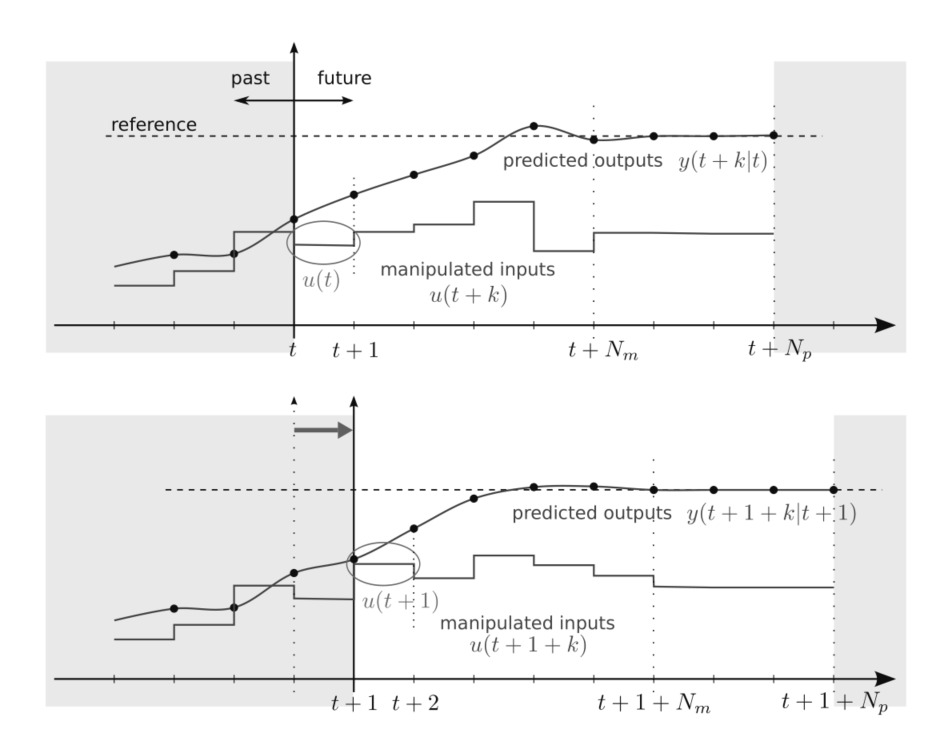
\includegraphics[width=.9\textwidth]{EMPC_PNG_Pics/RHC_gray.jpg}
        \caption{Graphycal display of receiding horison control (RHC) idea \cite{borrelli2017predictive}.}
        \label{BASICCSR:fig:RHC}
    \end{figure}

The Formulation of the optimal control problem with moving horizon \cite{goodwin2006constrained} in the system \ref{BASICMPC:equ:basic_LTI} with input and output constraints as mentioned in \ref{BASICMPC:equ:basic_LTI_constrained} with the cost function to minimize:
		
		\begin{equation}
        \begin{array}{rcl}
				J(\textbf{U},\textbf{x}(q))&=&\min_{\textbf{U}_{q\rightarrow q+N|q}}J_q(\textbf{x}(q),\textbf{U}_{q\rightarrow q+N|q})\\
                &=&\textbf{x}'_{q+N_y|q}\textbf{P}\textbf{x}_{q+N_y|q}+\sum^{N_y-1}_{k=0}\textbf{x}'_{q+k|q}\textbf{Q}\textbf{x}_{q+k|q}+\textbf{u}'_{q+k}\textbf{R}\textbf{u}_{q+k},\\
				&\textnormal{subj. to}&\textbf{x}_N\in\mathcal{X}_f,\textbf{x}_k\in\mathcal{X}^x,\textbf{u}_k\in\mathcal{U}^u\\
				&&\textbf{x}_{q|q}=\textbf{x}(q),\\
				&&\textbf{x}_{q+k+1|q}=\textbf{A}\textbf{x}_{q+k|q}+\textbf{B}\textbf{u}_{q+k},\\
				%&&\textbf{y}_{q+k|q}=\textbf{C}\textbf{x}_{q+k|q}, k\geq0,\\
				&&\textbf{u}_{q+k}=-K\textbf{x}_{q+k|q}, N_u\leq k\leq N_y,\\
        \end{array}
        \label{BASICMPC:equ:receiding_horison_problem}
    \end{equation}
		
		where $\textbf{Q}=\textbf{Q}'\geq0$, $\textbf{R}=\textbf{R}'\geq0$, $\textbf{P}\geq0$, $(\textbf{C},\textbf{A})$ is observable, and $N_u\leq N_y$, $N_c\leq N_y-1$. One trivial possibility to choose $K=0$ and $\textbf{P}$ to satisfy the Lyapunov equation:
		
		\begin{equation}
        \begin{array}{rcl}
				\textbf{P}&=&\textbf{A}'\textbf{PA}+\textbf{Q}\\
        \end{array}
        \label{BASICMPC:equ:receiding_horison_Lyapunov}
    \end{equation}
		
		This means that after $N_u$ samples the control stops and the system is evolving to an open loop form. It is obvious that the choice only makes sense if the open loop system is stable. The second option would as described with the method \ref{BASICMPC:equ:cost_function_Euclidian_recursive_twoP}, but this involves to use an unconstrained control for $N_u$ LQR samples. As a result, the MPC law calculates the optimal command sequence:
		
		\begin{equation}
        \begin{array}{rcl}
				\textbf{U}^*(q)&=&\left\{\textbf{u}^*_q,\dots,\textbf{u}^*_{q+N_u-1}\right\},\\
        \end{array}
        \label{BASICMPC:equ:receiding_optimal_sequence}
    \end{equation}
		
		and only the first control input is applied:
		
		\begin{equation}
        \begin{array}{rcl}
				\textbf{u}(q)=\textbf{u}^*_q.\\
        \end{array}
        \label{BASICMPC:equ:receiding_optimal_first}
    \end{equation}
		
		The optimal control inputs estimated for future samples are not taken into account and the algorithm is
repeated on the basis of new measurements or a new estimation of the states.	

    \subsubsection{Stability of MPC}\label{BASICCSR:sec:MPCStability}

    	The problem of closed system stability with the predictive control has been extensively studied e.g. in \cite{mayne2000constrained}, \cite{grieder2005stabilizing}. In the first generation of model based controllers, stability was achieved more experimentally by choosing parameters based on previous studies and experiences. In 1988 the Lyapunov stability method for discrete systems were introduced \cite{keerthi1988optimal}, and in 1990 for continuous systems \cite{mayne1990receding} also for continuous systems. \\
    While asymptotic convergence $\lim_{k\rightarrow\infty}\textbf{x}_k=0$ is a desirable property, it is generally not sufficient in practice. We would also like a system to stay in a small neighborhood of the origin when it is disturbed by a little. Formally this is expressed as Lyapunov stability.\\
    For the autonomous system:

    \begin{equation}
    \begin{array}{rcl}
            \textbf{x}_{k+1}&=&g(\textbf{x}_k)\\
            %&\textnormal{subj. to}&g(0)=0,
        \end{array}
        \label{BASICMPC:equ:autonom_system}
    \end{equation}

    where $g(0)=0$. The definition of Lyapunov stability is for the equilibrium point $\textbf{x}=0$ of system \ref{BASICMPC:equ:autonom_system} is:
    \begin{itemize}
    \item stable if, for each $\epsilon>0$, there is a $\varphi>0$ such that:
        \begin{equation}
        \begin{array}{c}
                \norm{\textbf{x}_0}<\varphi\textnormal{ s.t.: }\norm{\textbf{x}_k}<\epsilon,\textnormal{ }\forall k\geq0.
            \end{array}
            \label{BASICMPC:equ:lyapunov_1}
        \end{equation}

    \item unstable if not stable

    \item asymptotically stable if in the set $\boldsymbol{\Omega}\subseteq\mathbb{R}^n$ if its stable and:
       \begin{equation}
        \begin{array}{c}
                \lim_{k\rightarrow\infty}\textbf{x}_k=0,\textnormal{ }\forall\textbf{x}_0\in\boldsymbol{\Omega}.
            \end{array}
            \label{BASICMPC:equ:lyapunov_2}
        \end{equation}

    \item globally asymptotically stable if it is asymptotically stable and $\boldsymbol{\Omega}=\mathbb{R}^n$

    \item exponentially stable if it is stable and there exist constants $\chi>0$ and $\psi\in(0,1)$ such that:
    \begin{equation}
        \begin{array}{c}
                \norm{\textbf{x}_0}<\varphi\textnormal{ s.t.: }\norm{\textbf{x}_k}\leq\chi\norm{\textbf{x}_0}\psi^k,\textnormal{ }\forall k\geq0.
            \end{array}
            \label{BASICMPC:equ:lyapunov_3}
        \end{equation}


    \end{itemize}

    Usually to show Lyapunov stability of the origin for a particular system one constructs a so called Lyapunov function, i.e., a function satisfying the conditions of the following theorem:\\
    Consider the equilibrium point $\textbf{x}=0$ of system \ref{BASICMPC:equ:autonom_system}. Let $\boldsymbol{\Omega}\subset\mathbb{R}^n$ be a closed and bounded set containing the origin. Assume there exists a function $V:\mathbb{R}^n\rightarrow\mathbb{R}$ continuous at the origin, finite for every $\textbf{x}\in\boldsymbol{\Omega}$ and such that:

    \begin{subequations}
    \label{BASICMPC:equ:lyapunov_4_1}
        \begin{align}
                V(0)=0 \label{BASICMPC:equ:lyapunov_4_1_a}\\
                V(\textbf{x})>0,\textnormal{ }\forall\textbf{x}\in\boldsymbol{\Omega}\textbackslash\{0\} \label{BASICMPC:equ:lyapunov_4_1_b}\\
                V(\textbf{x}_{k+1})-V(\textbf{x}_{k})\leq-\chi(\textbf{x}_k),\textnormal{ }\forall\textbf{x}\in\boldsymbol{\Omega}\textbackslash\{0\}, \label{BASICMPC:equ:lyapunov_4_1_c}
        \end{align}
    \end{subequations}

     where $\chi:\mathbb{R}^n\rightarrow\mathbb{R}$ is a continuous positive definite function, then $\textbf{x}=0$ is asymptotically stable. As such a function satisfying \ref{BASICMPC:equ:lyapunov_4_1} is called a Lyapunov function.\\
     A similar theorem can be derived for global asymptotic stability i.e.: $\boldsymbol{\Omega}=\mathbb{R}^n$:
     Consider the equilibrium point $\textbf{x}=0$ of system \ref{BASICMPC:equ:autonom_system}. Let $\boldsymbol{\Omega}\subset\mathbb{R}^n$ be a closed and bounded set containing the origin. Assume there exists a function $V:\mathbb{R}^n\rightarrow\mathbb{R}$ continuous at the origin, finite for every $\textbf{x}\in\boldsymbol{\Omega}$ and such that:

     \begin{subequations}
    \label{BASICMPC:equ:lyapunov_4_2}
        \begin{align}
                \norm{\textbf{x}}\rightarrow\infty,\textnormal{ s.t.: }V(\textbf{x})\rightarrow\infty \label{BASICMPC:equ:lyapunov_4_2_a}\\
                V(0)=0 \label{BASICMPC:equ:lyapunov_4_2_b}\\
                V(\textbf{x})>0,\textnormal{ }\forall\textbf{x}\neq0 \label{BASICMPC:equ:lyapunov_4_2_c}\\
                V(\textbf{x}_{k+1})-V(\textbf{x}_{k})\leq-\chi(\textbf{x}_k),\textnormal{ }\forall\textbf{x}\neq0, \label{BASICMPC:equ:lyapunov_4_2_d}
            \end{align}
            \end{subequations}
     where $\chi:\mathbb{R}^n\rightarrow\mathbb{R}$ is a continuous positive definite function, then $\textbf{x}=0$ is globally asymptotically stable.\\
     For linear systems a simple and effective Lyapunov function can be:

     \begin{equation}
        \begin{array}{rcl}
                V(\textbf{x})&=&\textbf{x}'\textbf{P}\textbf{x},\textbf{P}\succ 0,\\
            \end{array}
            \label{BASICMPC:equ:lyapunov_5}
        \end{equation}

    In order to test the satisfaction of the last point of \ref{BASICMPC:equ:lyapunov_4_2}, we compute:

    \begin{equation}
        \begin{array}{rcl}
                V(\textbf{x}_{k+1})-V(\textbf{x}_{k})&=&\textbf{x}'_{k+1}\textbf{P}\textbf{x}_{k+1}-\textbf{x}'_{k}\textbf{P}\textbf{x}_{k}\\
                &=&\textbf{x}'_{k}(\textbf{A}'\textbf{P}\textbf{A})\textbf{x}_{k}-\textbf{x}'_{k}\textbf{P}\textbf{x}_{k}\\
                &=&\textbf{x}'_{k}(\textbf{A}'\textbf{P}\textbf{A}-\textbf{P})\textbf{x}_{k},
            \end{array}
            \label{BASICMPC:equ:lyapunov_6}
        \end{equation}

    therefore, if \ref{BASICMPC:equ:lyapunov_5} holds true then:

    \begin{equation}
        \begin{array}{rcl}
                 \textbf{A}'\textbf{P}\textbf{A}-\textbf{P}&=&-\textbf{Q},\textbf{Q}\succ 0,\\
            \end{array}
            \label{BASICMPC:equ:lyapunov_7}
        \end{equation}

which is referred as discrete time Lyapunov equation.

\section[Predictive control of a CSR]{Constrained, explicit predictive control for current source buck-type rectifiers}\label{EMPC:sec:main}

As mentioned in section \oldref{BASICCSR:sec:CSR} current source rectifiers (CSR) play a major role in industrial instrumentation. They are invaluable, in the fields of direct power control, torque control, or power injection is required. In this chapter, the modeling and control of such CSR (or buck-type rectifiers), in a model based predictive manner, with explicit partitioning of the state space. The reason of the regular MPC's insufficiency is that power electronic systems require very low time constant to operate smoothly. As such pre-mapping the state-space with applicable control rules gives a great leverage, thus making the possible computational unit much cheaper.
		
\subsection{Modeling}\label{EMPC:sec:Modeling}

Understandably, model based controllers require the system's model the ought to control, or supervise. In this case the most common structure of a CSR is chosen, with inductive and capacitive filtering on both ends. The differential equations are constructed based on Kirchoff's law and then presented as a state space model for further examination.

\subsubsection{Mathematical modeling of the CSR}\label{EMPC:sec:ModelofCSR}

    The structure of the classical three phase buck-type current source rectifier (CSR) is presented in \ref{EMPC:fig:network}. In continuous current mode, the differential equations corresponding to the CRS’s inductor currents and capacitor voltages are the following:

    \begin{figure}[!ht]
        \centering
        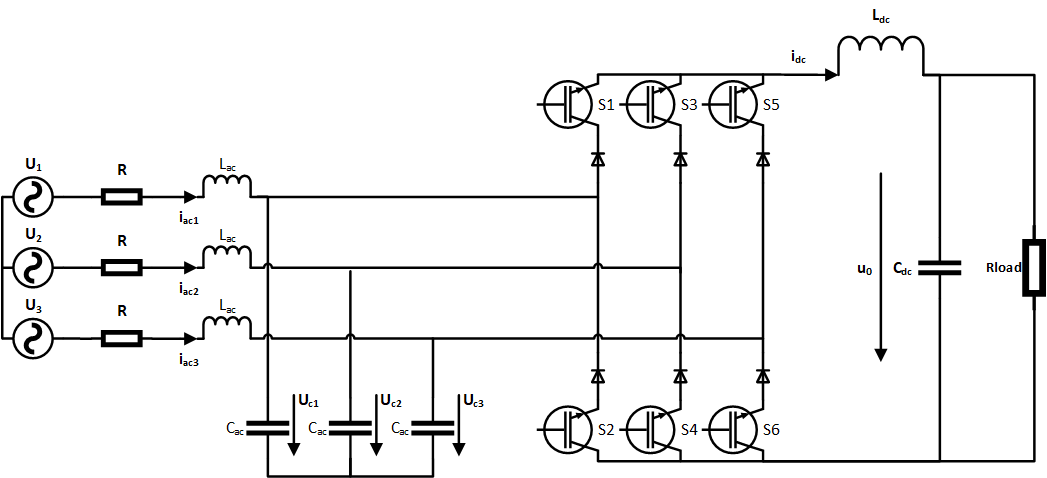
\includegraphics[width=\textwidth]{EMPC_PNG_Pics/circuit.png}
        \caption{Circuit diagram of the three-phase buck-type rectifier with insulated gate bipolar transistors (IGBTs).}
        \label{EMPC:fig:network}
    \end{figure}
		
        \begin{equation}
        \begin{array}{rcl}
            L_{ac}\dot{i_{ac_p}}&=&u_p-u_{c_p}-Ri_{ac_p}\\
            C_{ac}\dot{u_{c_p}}&=&i_{ac_p}-\delta_pi_{dc}\\
            L_{dc}\dot{i_{dc}}&=&(\sum_{p=1}^{3}\delta_pu_{c_p})-u_0\\
            C_{dc}\dot{u_0}&=&i_{dc}-\frac{u_0}{R_{load}}\\
        \end{array}
        \label{EMPC:equ:abc_eqn}
    \end{equation}

    where $p\in\{1,2,3\}$ is the index of three phases and $\delta_p$ describes the conduction state of the rectifier leg p \ref{EMPC:equ:delta_set}.

    \begin{equation}
        \begin{array}{rcl}
            \delta_p&=&\begin{Bmatrix}
                \textrm{1 if the upper transitor is ON}\\
                \textrm{-1 if the lower transistor is ON}\\
                \textrm{0 if both are ON or OFF}
            \end{Bmatrix}
        \end{array}
        \label{EMPC:equ:delta_set}
    \end{equation}

    Converting the components in the stationary (Clarke) frame (displayed in section \oldref{BASICCSR:sec:Clarke}) of the space phasors of the three-phase quantities, from \ref{EMPC:equ:abc_eqn} it results:

    \begin{equation}
        \begin{array}{rcl}
            L_{ac}\dot{i_{ac_\alpha}}&=&u_\alpha-u_{c_\alpha}-Ri_{ac_\alpha}\\
            L_{ac}\dot{i_{ac_\beta}}&=&u_\beta-u_{c_\beta}-Ri_{ac_\beta}\\
            C_{ac}\dot{u_{c_\alpha}}&=&i_{ac_\alpha}-\delta_\alpha i_{dc}\\
            C_{ac}\dot{u_{c_\beta}}&=&i_{ac_\beta}-\delta_\beta i_{dc}\\
            L_{dc}\dot{i_{dc}}&=&1.5(\delta_\alpha u_{c_\alpha}+\delta_\beta u_{c_\beta})-u_0\\
            C_{dc}\dot{u_0}&=&i_{dc}-\frac{u_0}{R_{load}}\\
        \end{array}
        \label{EMPC:equ:abc_alfabeta}
    \end{equation}

    Equation \ref{EMPC:equ:abc_alfabeta} is transformed to the synchronous reference (Park) frame (displayed in section \oldref{BASICCSR:sec:Park}) rotating with the $u_{c_d}$ capacitor voltage space vector. The resulting mathematical model is thus:

    \begin{equation}
        \begin{array}{rcl}
            L_{ac}\dot{i_{ac_d}}&=&u_d-u_{c_d}-Ri_{ac_d}+\omega_s L_{ac}i_{ac_q}\\
            L_{ac}\dot{i_{ac_q}}&=&u_d-u_{c_q}-Ri_{ac_q}-\omega_s L_{ac}i_{ac_d}\\
            C_{ac}\dot{u_{c_d}}&=&i_{ac_d}-\delta_di_{dc}+\omega_s C_{ac}u_{c_q}\\
            C_{ac}\dot{u_{c_q}}&=&i_{ac_q}-\delta_qi_{dc}-\omega_s C_{ac}u_{c_d}\\
            L_{dc}\dot{i_{dc}}&=&1.5(\delta_d u_{c_d}+\delta_q u_{c_q})-u_0\\
            C_{dc}\dot{u_0}&=&i_{dc}-\frac{u_0}{R_{load}}\\
        \end{array}
        \label{EMPC:equ:abc_dq}
    \end{equation}

    where $\omega_s$ represents the network voltage vector’s angular velocity.

    \subsubsection{Model simplification}\label{EMPC:sec:Simplification}

    Notice, that the sixth-order ODE model \ref{EMPC:equ:abc_dq} is bilinear in its states and
    inputs because of the product terms (e.g.: $\delta_di_{dc}$). As such, using design methods for linear systems is not straightforward. The high complexity given by the system’s order is another problem to tackle. For designing classic MPC, linear, low-order equation systems are favorable. Hence simplification of the model would bring noteworthy benefits, making the MPC design more straightforward, when a linear system resulted.
    Since the three phase alternating current (AC) and the direct current (DC) side’s time constants differ significantly (as in the AC: $\omega_{ac}=\frac{1}{\sqrt{L_{ac} C_{ac}}}\cong5.7\cdot10^3$ rad/s, and on the DC: $\omega_{dc}=\frac{1}{\sqrt{L_dc C_dc}}\cong2.8\cdot10^2$ rad/s, see Table \ref{EMPC:tbl:params}. for reference). Thus, the differential equations can be separated into two sets, and the control of the AC and DC sides can be decoupled as described in \cite{ahmed2014model}. The AC side model results as follows:


    \begin{equation}
        \begin{array}{rcl}
            \begin{bmatrix}
                \dot{i_{ac_d}}\\
                \dot{i_{ac_q}}\\
                \dot{u_{c_d}}\\
                \dot{u_{c_q}}
            \end{bmatrix}&=&
            \begin{bmatrix}
                -\frac{R}{L_{ac}}   &\omega &-\frac{1}{L_{ac}}  &0\\
                -\omega   &-\frac{R}{L_{ac}} &0  &-\frac{1}{L_{ac}}\\
                \frac{1}{C_{ac}}   &0 &0  &\omega\\
                0   &\frac{1}{C_{ac}} &-\omega  &0
            \end{bmatrix}
            \begin{bmatrix}
                i_{ac_d}\\
                i_{ac_q}\\
                u_{c_d}\\
                u_{c_q}
            \end{bmatrix}+
            \begin{bmatrix}
                \frac{u_d}{L_{ac}}\\
                \frac{u_q}{L_{ac}}\\
                -\frac{\delta_di_{dc}}{C_{ac}}\\
                -\frac{\delta_qi_{dc}}{C_{ac}}
            \end{bmatrix}
        \end{array}
        \label{EMPC:equ:mtx_AC}
    \end{equation}

    Looking at the state matrix it can be further stated that there are only weak couplings between the $d$ and $q$ synchronous reference frame components. This allows to handle them separately, and later to design separate control for each.
    The equation system describing the DC side dynamics is the following:

    \begin{equation}
        \begin{array}{rcl}
            \begin{bmatrix}
                \dot{i_{dc}}\\
                \dot{u_{0}}
            \end{bmatrix}&=&
            \begin{bmatrix}
                0&  -\frac{1}{L_{dc}}\\
                \frac{1}{C_{dc}}&   -\frac{1}{R_{load}C_{dc}}
            \end{bmatrix}
            \begin{bmatrix}
                i_{dc}\\
                u_0
            \end{bmatrix}+
            \begin{bmatrix}
                \frac{1.5}{L_{dc}}(\delta_du_{c_d}+\delta_qu_{c_q})\\
                0
            \end{bmatrix}
        \end{array}
        \label{EMPC:equ:mtx_DC}
    \end{equation}

    It can be noticed that, with the AC and DC model separation, bilinearity disappears, since the binding coefficients are present only in the input $(\textbf{u})$ of the DC state space model \ref{EMPC:equ:mtx_DC}. Consequently, all equations are linear and with a considerably lower order, making control design much easier and allowing for the application of linear design methods. For the DC side dynamics, the linear time invariant differential equation system’s matrices can be identified for predictive control design purposes:

    \begin{equation}
        \begin{array}{rcl}
            \textbf{x}&=&\begin{bmatrix}
                i_{dc}\\
                u_0
            \end{bmatrix},\\
            \textbf{u}&=&(\delta_d u_{c_d}+\delta_q u_{c_d}),\\
            \textbf{y}&=&u_0,\\
            \textbf{A}&=&\begin{bmatrix}
                0&  -\frac{1}{L_{dc}}\\
                \frac{1}{C_{dc}}&   -\frac{1}{R_{load}C_{dc}}
            \end{bmatrix},\\
            \textbf{B}&=&\begin{bmatrix}
                i_{dc}\\
                u_0
            \end{bmatrix},\\
            \textbf{C}&=&\begin{bmatrix}0 &1\end{bmatrix}.
        \end{array}
        \label{EMPC:equ:mtx_ctrl}
    \end{equation}

    where \textbf{x}, \textbf{u} and \textbf{y} are the state, input and output vectors of the DC-side system, and \textbf{A}, \textbf{B} and \textbf{C} are the state, input and output matrices.
    The circuit parameters used for the implementation of the control structure based on this model are presented in Table \ref{EMPC:tbl:params}.

    \begin{table}[]
    \center
		\caption{The applied parameters in model and controller design}
        \begin{tabular}{|l|l|}
        \hline
        Parameter      & Value  \\ \hline
        \textbf{R}     & 0.3 $\Omega$ \\ \hline
        \textbf{Rload} & 10 $\Omega$  \\ \hline
        \textbf{Lac}   & 1 mH    \\ \hline
        \textbf{Ldc}   & 30 mH   \\ \hline
        \textbf{Cac}   & 30 $\mu$F   \\ \hline
        \textbf{Cdc}   & 400 $\mu$F  \\ \hline
        \textbf{f}     & 50 Hz   \\ \hline
        \textbf{fpwm}  & 20 kHz  \\ \hline
        \textbf{Un}    & 400 V   \\ \hline
        \end{tabular}
        \label{EMPC:tbl:params}
    \end{table}

\subsubsection{Control structure}\label{EMPC:sec:ControlStruct}

    Using the separation of the AC side and DC side controllers, the control structure depicted in Fig. \ref{EMPC:fig:ControlStruct}. is proposed.

    \begin{figure}[!ht]
        \centering
        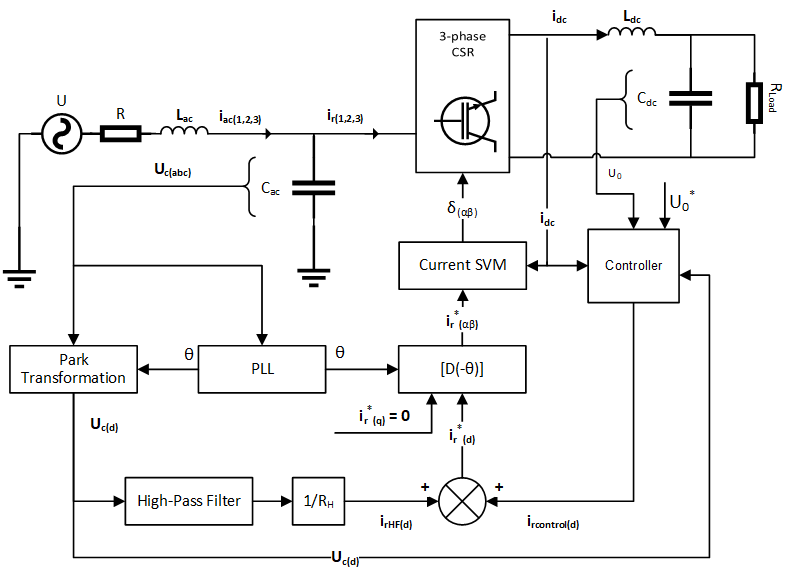
\includegraphics[width=\textwidth]{EMPC_PNG_Pics/ControlStructure.png}
        \caption{Block diagram of the control structure.}
        \label{EMPC:fig:ControlStruct}
    \end{figure}

    The controllers operate in the synchronous frame of the AC filter capacitor voltages $u_{c_{(1,2,3)}}$, and the rectifier input currents $i_{r_{(1,2,3)}}$ are in phase with the capacitor voltages.
    The current reference $i^*_{\alpha\beta}$ supplied to the space vector modulation unit in the stationary frame, is obtained by coordinate transformation $[D(-\Theta)]$ (or Park to Clarke transformation) of the current reference \ref{EMPC:equ:sync_ctrl} delivered by the current controllers in the synchronous frame.

    \begin{equation}
        \begin{array}{rcl}
            \begin{Bmatrix}
                i^*_{r_d}=i_{rcontrol_d}+i_{rHF_d}\\
                i^*_{r_q}=0
            \end{Bmatrix}
        \end{array}
        \label{EMPC:equ:sync_ctrl}
    \end{equation}

    In \ref{EMPC:equ:sync_ctrl}, $i_{rcontrol_d}$ represents the output of the DC voltage controller, while $i_{rHF_d}$ represents the damping current, proportional with the high frequency component of the filter capacitor voltage (the fundamental component of the capacitor voltage in the stationary frame becomes a DC component in the synchronous frame). The DC and AC side control units are explained in more detail in the following sections, and the performance of the control structure is evaluated.
		
\subsection{Control}\label{EMPC:sec:Control}

    In this section the model based control algorithm is explained, used on the DC side, followed by a simpler AC side active damping.

\subsubsection{DC-side explicit model predictive control} \label{EMPC:sec:DCside}

    Model predictive control (MPC) is an efficient and systematic method for solving complex multi-variable constrained optimal control problems \cite{vajda2017limiting}. The basic notions of MPC is explained in section \oldref{BASICCSR:sec:MPC}, where the MPC control law is explained, namely, is based on the “receding horizon formulation”, where the model’s assumed behavior is calculated for a number of $N$ steps, where $N$ stands for the horizon’s length. Only the first step of the computed optimal input is applied in each iteration. The remaining steps of the optimal control input are discarded and a new optimal control problem (explained in section \oldref{BASICCSR:sec:LQR}) is solved at the next sample time. Using this approach, the receding horizon policy provides the controller with the desired feedback characteristics, although with high order systems the computational effort is considerably demanding since all the steps should be taken in to account on the specified horizon in every iteration.\\
		With Explicit MPC (EMPC), the discrete time constrained optimal control problem is reformulated as multi-parametric linear or quadratic programming. As explained in section \oldref{BASICCSR:sec:OptimalControl}, the optimization problem can be solved offline, making it much more feasible from the perspective of the optimal control task. The optimal control law is a piecewise affine function of the states, and the resulting solution is stored in a pre-calculated lookup table. The parameter space, or the state-space is partitioned into critical regions. The real-time implementation consists in searching for the active critical region, where the measured state variables lie, and in applying the corresponding piecewise affine control law to achieve the desired dynamics.
    In order to introduce the MPC implementation, let us consider a linear discrete time system \ref{EMPC:equ:DiscreteStateSpace} derived with the discretisation of system \ref{EMPC:equ:mtx_DC} with zero-order hold method, where control inputs are assumed piecewise constant over the simulation sample time $T_s=\frac{1}{f_s}$ :

    \begin{equation}
        \begin{array}{rcl}
            \textbf{x}(t+1)&=&\textbf{A}_d\textbf{x}(t)+\textbf{B}_d\textbf{u}(t)\\
            \textbf{y}(t)&=&\textbf{C}_d\textbf{x}(t)
        \end{array}
        \label{EMPC:equ:DiscreteStateSpace}
    \end{equation}

    where $\textbf{A}_d$, $\textbf{B}_d$, $\textbf{C}_d$ are the matrices of the discretised system derived from \ref{EMPC:equ:mtx_ctrl}. With system \ref{EMPC:equ:DiscreteStateSpace} is linear and time invariant, MPC design can be followed. The following constraints have to be satisfied:

    \begin{equation}
        \begin{array}{r}
            \textbf{y}_{min}\leq\textbf{y}(t)\leq\textbf{y}_{max},\\
            \textbf{u}_{min}\leq\textbf{u}(t)\leq\textbf{u}_{max}
        \end{array}
        \label{EMPC:equ:contraint_desc}
    \end{equation}

    where $t>0$, $\textbf{x}\in \mathbb{R}^n$, $\textbf{u}\in \mathbb{R}^m$, $\textbf{y}\in \mathbb{R}^p$. The MPC solves the following constrained optimization problem \cite{rivera2013predictive}:

    \begin{equation}
        \begin{array}{rcl}
           \displaystyle \min_{U=\{u_t\dots u_t+N_u-1\}}J(\textbf{u},\textbf{x}(t))&=&\sum^{N_y-1}_{k=0}(\textbf{x}^T_{t+N_y|t}\textbf{Q}\textbf{x}_{t+N_y|t}+
           \textbf{u}^T_{t+k}\textbf{R}\textbf{u}_{t+k})\\
        \end{array}
        \label{EMPC:equ:optim_problem}
    \end{equation}

    subject to:

    \begin{equation}
        \begin{array}{l}
            \textbf{x}_{min}\leq\textbf{x}_{t+k|t}\leq\textbf{x}_{max},\,k=1,\dots,N_c-1\\
            \textbf{u}_{min}\leq\textbf{u}_{t+k|t}\leq\textbf{u}_{max},\,k=1,\dots,N_c-1\\
            \textbf{x}_{t|t}=\textbf{x}(t),\,\textbf{u}_{t|t}=\textbf{u}(t)\\
            \textbf{x}_{t+k+1|t}=\textbf{A}_d\textbf{x}_{t+k|t}+\textbf{B}_d\textbf{u}_{t+k|t}\\
            \textbf{y}_{t+k|t}=\textbf{C}_d\textbf{x}_{t+k|t}\\
            \textbf{u}_{t+k|t}=-K\textbf{x}_{t+k|t},\,k\geq0\\
        \end{array}
        \label{EMPC:equ:optim_problem_constr}
    \end{equation}
There the formulation of such problem is described in detail in chapter \ref{BASICCSR:sec:OptimalControl}.\\
    This problem is solved at each time instant $t$, where $\textbf{x}_{t+k\vert t}$ denotes the state vector predicted at time $t+k$, obtained by applying the input sequence $\textbf{u}_{t|t}...\textbf{u}_{t|t+1}$ to model \ref{EMPC:equ:quadratic_regions}, starting from the state $\textbf{x}_{t|t}$. Further, it is assumed that $Q$ and $R$, are symmetric positive semidefinite $(\textbf{Q}_w=\textbf{Q}_w^T\geq0$, $\textbf{R}_w=\textbf{R}_w^T>0)$ and $K$ is a feedback gain. Further, $N_y,N_u,N_c$ are the output, input and constraint horizons, respectively.
    Using the model for predicting the future behavior of the system and with some appropriate substitution and variable manipulation which basic notions showed in section \oldref{BASICCSR:sec:MPC}, the problem \ref{EMPC:equ:optim_problem},\ref{EMPC:equ:optim_problem_constr} can be transformed to the standard multi parametric quadratic programming form, as described in \cite{rivera2013predictive}:
%
%    \begin{equation}
%        \begin{array}{rcl}
%            J(\textbf{x}(t))&=&\min \textbf{z}'\textbf{H}\textbf{z}
%        \end{array}
%        \label{EMPC:equ:quadratic_program}
%    \end{equation}

    \begin{equation}
        \begin{array}{rcl}
            J^*(\textbf{x}(t))&=&\min_{\textbf{z}}J(\textbf{x},\textbf{z})=\frac{1}{2}\textbf{z}'\textbf{H}\textbf{z}
        \end{array}
        \label{EMPC:equ:quadratic_program}
    \end{equation}

    where subject to:

    \begin{equation}
        \begin{array}{rcl}
            \textbf{Gz}&\leq&\textbf{w}+\textbf{S}\textbf{x}(t)
        \end{array}
        \label{EMPC:equ:quadratic_inequality}
    \end{equation}

    where the matrices $\textbf{H}$, $\textbf{G}$, $\textbf{w}$, $\textbf{S}$ result directly from the coordinate transformations described in \ref{BASICCSR:sec:OptimalControl}. The solution of the quadratic optimization problem for each critical region has the form:

    \begin{equation}
        \begin{array}{rcl}
            \textbf{u}^*&=&\textbf{F}_i\textbf{x}+\textbf{g}_i
        \end{array}
        \label{EMPC:equ:quadratic_regions}
    \end{equation}

    and the critical region is described by:

    \begin{equation}
        \begin{array}{rcl}
            \mathcal{C}_{reg_i}&=&\{\textbf{x}\in \mathbb{R}^n|\textbf{H}_i\textbf{x}\leq \textbf{K}_i\}
        \end{array}
        \label{EMPC:equ:quadratic_critical}
    \end{equation}

    Thus, the explicit MPC controller is completely characterized by the set of parameters:

    \begin{equation}
        \begin{array}{l}
            \{\textbf{F}_i,\textbf{g}_i,\textbf{H}_i,\textbf{K}_i|i=1\dots N\}
        \end{array}
        \label{EMPC:equ:quadratic_set}
    \end{equation}

    In case of the discrete time system resulting from \ref{EMPC:equ:mtx_ctrl}, for sampling time equal with the switching period $T_s=5\cdot10^{-5}$  s, the problem defined to be solved by MPC is the minimization of the quadratic cost function \ref{EMPC:equ:DiscreteStateSpace} for:

    \begin{equation}
        \begin{array}{l}
            \textbf{R}_w=\begin{bmatrix}
                1& 0\\
                0& 1\\
            \end{bmatrix},
            \textbf{Q}_w=\begin{bmatrix}
                10^{-6}& 0\\
                0& 10^{-6}\\
            \end{bmatrix},
            N_y=N_u=N_c=2
        \end{array}
        \label{EMPC:equ:quadratic_mtx_set}
    \end{equation}

    Since $N_y,N_u,N_c$ take the same value, they will be substituted by $N$.
    The constraints defined based on the rated power of the CSR $P_n=2500$ W, are:

    \begin{equation}
        \begin{array}{rcl}
            0\leq&i_{dc}&\leq 50A\\
            0\leq&u_{0}&\leq 500V
        \end{array}
        \label{EMPC:equ:numeric_constraints}
    \end{equation}

    The state space partition resulting from this problem has 13 critical regions, which can be observed in Fig. \ref{EMPC:fig:regions}.

    \begin{figure}[!ht]
        \centering
        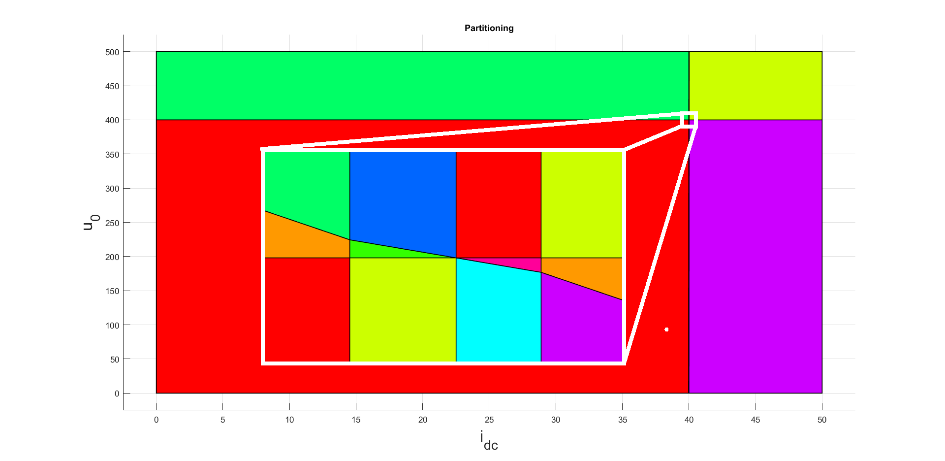
\includegraphics[width=\textwidth]{EMPC_PNG_Pics/Regions.png}
        \caption{State space partitioning.}
        \label{EMPC:fig:regions}
    \end{figure}

    From the basis of the discretised model \ref{EMPC:equ:DiscreteStateSpace}, the given constraints \ref{EMPC:equ:numeric_constraints}, and horizon \ref{EMPC:equ:numeric_constraints} the cost function \ref{EMPC:equ:optim_problem} is established via the MPT toolbox [30] and used in the generated controller for the EMPC design [29], [31]. The controller is created as a compliable S-function in the Matlab/Simulink environment and its place in the control structure can be observed in Fig. \ref{EMPC:fig:MPCStructure}. as the EMPC controller.
    The output of the MPC controller is the control variable obtained via solving \ref{EMPC:equ:optim_problem_constr} and
    $u_{MPC}=(\delta_du_{c_d}+\delta_qu_{c_q})$, from which the current reference can be calculated using \ref{EMPC:equ:numeric_constraints}. The quadrature component $u_{c_q}$ is zero in the synchronous frame of the filter capacitor voltage.


    \begin{equation}
        \begin{array}{rcl}
            i_{rMPC_{d}}&=&\frac{u_{MPC}}{u_{c_d}}\cdot i_{dc}
        \end{array}
        \label{EMPC:equ:direct_controlval}
    \end{equation}

    \begin{figure}[!ht]
        \centering
        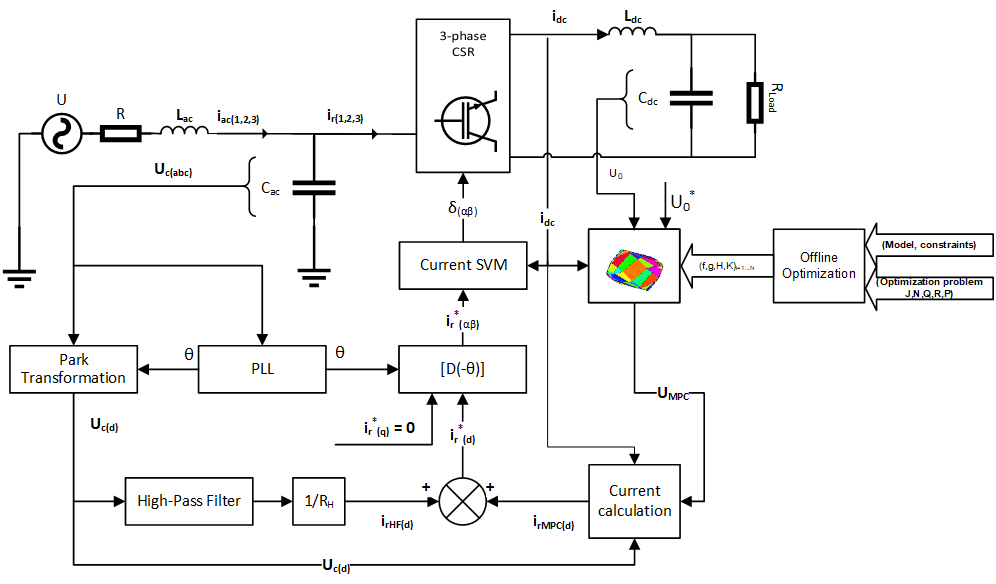
\includegraphics[width=\textwidth]{EMPC_PNG_Pics/MPCStructure.png}
        \caption{The control structure of the CSR, with MPC controller on the DC side.}
        \label{EMPC:fig:MPCStructure}
    \end{figure}

\subsubsection{Active AC-side damping}\label{EMPC:sec:ACdamping}

    The CSR requires a voltage supply on the AC side. Taking the inductive character of the mains into consideration, the presence of a three-phase capacitor bank at the input of the CSR is a must. The most convenient is to use three-phase LC filtering with inductors on the lines and star connected capacitors resembling those in Fig. \ref{EMPC:fig:network}, although the resonance phenomena between these components can still cause difficult problems. The simplest way to dampen the resonance on the AC side LC filter is to add a damping resistor across the capacitor \cite{regaya2014new}. Because these resistors result in high losses, active damping methods have been proposed, which emulate damping resistors by control. This makes the CSR bridge produce an additional high frequency current, equivalent to the presence of virtual damping resistors connected in parallel with the AC capacitors. The resonance of the AC side LC filter produces harmonics in the capacitor voltage with frequency close to $\omega_{ac}=\frac{1}{\sqrt{L_{ac}C_{ac}}}$, which appears as $\omega_{ac}-\omega$ component in $u_{c_d}$, where $\omega=2\pi f$. The fundamental component of the capacitor voltage represents a DC component in the synchronous reference frame. Therefore, a high-pass filter (HPF) is applied to filter out this DC component, with the transfer function:

    \begin{equation}
        \begin{array}{rcl}
            HPF(s)&=&\frac{s}{s+0.1\cdot(\omega_{ac}-\omega}
        \end{array}
        \label{EMPC:equ:AC_HPF}
    \end{equation}

    A virtual damping resistance $R_H$ has been defined for calculation of the damping current component $i_{HPF}$ from the HPF component of the capacitor voltage.

\subsection{Modulation}\label{EMPC:sec:Modulation}

    The chosen modulation strategy is developed in the $"\alpha\beta"$ stationary reference frame, based on the notions already mentioned in section \oldref{BASICCSR:sec:OperationPrinciple}. The structure requires simultaneous conduction of the upper and lower transistors of the bridge, since the current of the $L_{dc}$  choke must not be interrupted. Additionally, the switching devices are considered as ideal.

    \begin{figure}[!ht]
        \centering
        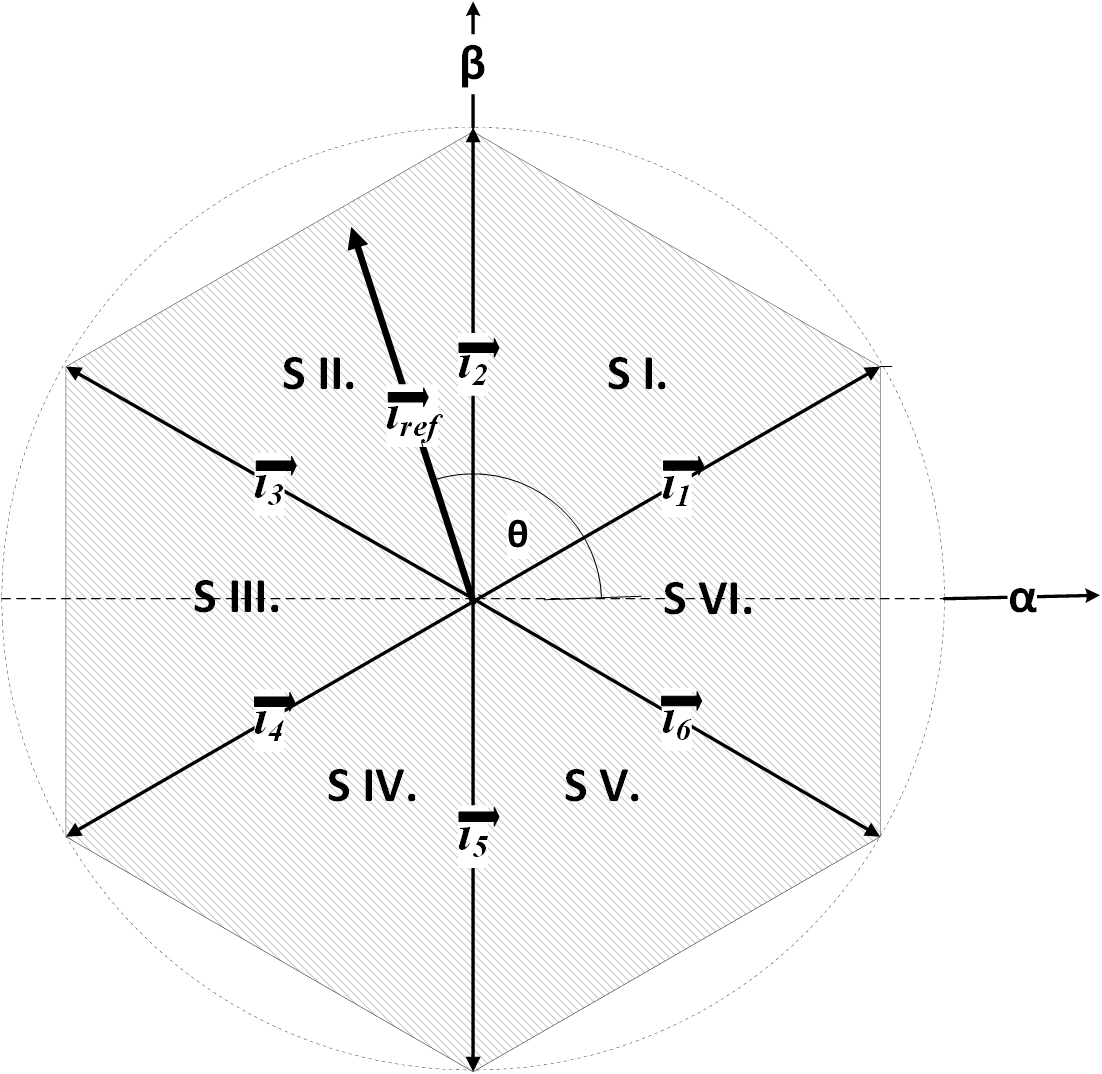
\includegraphics[width=.6\textwidth]{EMPC_PNG_Pics/VectorPhasor.png}
        \caption{The fundamental input current vectors corresponding to the active switching states of the CSR.}
        \label{EMPC:fig:VectorPhasor}
    \end{figure}

    According to this, one of the upper and one of the lower switches must be closed at all times. This allows nine states, six of which are active. There are three "zero" vectors, corresponding to the switching states, when both devices of one of the bridge legs are in conduction. These current vectors are shown in Table \ref{EMPC:tbl:fundamental_vect}.


% Please add the following required packages to your document preamble:
% \usepackage{multirow}
% \usepackage[table,xcdraw]{xcolor}
% If you use beamer only pass "xcolor=table" option, i.e. \documentclass[xcolor=table]{beamer}

\begin{table}[]
\caption{The fundamental input current vectors corresponding to the active switching states of the CSR.}
    \begin{tabular}{|l|l|l|l|l|l|l|l|l|l|l|}
    \hline
    \rowcolor[HTML]{EFEFEF}
    \multicolumn{1}{|c|}{\cellcolor[HTML]{EFEFEF}}                                & \multicolumn{6}{c|}{\cellcolor[HTML]{EFEFEF}\textbf{Switching State}}       & \multicolumn{3}{l|}{\cellcolor[HTML]{EFEFEF}\textbf{Phase currents}} & \multicolumn{1}{c|}{\cellcolor[HTML]{EFEFEF}}                                                 \\ \cline{2-10}
    \rowcolor[HTML]{EFEFEF}
    \multicolumn{1}{|c|}{\multirow{-2}{*}{\cellcolor[HTML]{EFEFEF}\textbf{Name}}} & \textbf{1} & \textbf{2} & \textbf{3} & \textbf{4} & \textbf{5} & \textbf{6} & \textbf{ia}           & \textbf{ib}           & \textbf{ic}          & \multicolumn{1}{c|}{\multirow{-2}{*}{\cellcolor[HTML]{EFEFEF}\textbf{Vector representation}}} \\ \hline
    $\vec{i}_1$                                                                           & 1          & 0          & 0          & 0          & 0          & 1          & $i_{dc}$                   & 0                     & -$i_{dc}$                 & $2i_{dc}e^{j\pi/6}/\sqrt{3}$                                                                                           \\ \hline
    $\vec{i}_2$                                                                            & 0          & 0          & 1          & 0          & 0          & 1          & 0                     & $i_{dc}$                   & -$i_{dc}$                 & $2i_{dc}e^{j\pi/2}/\sqrt{3}$                                                                                           \\ \hline
    $\vec{i}_3$                                                                            & 0          & 1          & 1          & 0          & 0          & 0          & -$i_{dc}$                  & $i_{dc}$                   & 0                    & $2i_{dc}e^{j5\pi/6}/\sqrt{3}$                                                                                          \\ \hline
    $\vec{i}_4$                                                                            & 0          & 1          & 0          & 0          & 1          & 0          & -$i_{dc}$                  & 0                     & $i_{dc}$                  & $2i_{dc}e^{j7\pi/6}/\sqrt{3}$                                                                                          \\ \hline
    $\vec{i}_5$                                                                           & 0          & 0          & 0          & 1          & 1          & 0          & 0                     & -$i_{dc}$                  & $i_{dc}$                  & $2i_{dc}e^{j3\pi/2}/\sqrt{3}$                                                                                           \\ \hline
    $\vec{i}_6$                                                                            & 1          & 0          & 0          & 1          & 0          & 0          & $i_{dc}$                   & -$i_{dc}$                  & 0                    & $2i_{dc}e^{j11\pi/6}/\sqrt{3}$                                                                                           \\ \hline
    $\vec{i}_7$                                                                            & 1          & 1          & 0          & 0          & 0          & 0          & 0                     & 0                     & 0                    & 0                                                                                             \\ \hline
    $\vec{i}_8$                                                                            & 0          & 0          & 1          & 1          & 0          & 0          & 0                     & 0                     & 0                    & 0                                                                                             \\ \hline
    $\vec{i}_9$                                                                            & 0          & 0          & 0          & 0          & 1          & 1          & 0                     & 0                     & 0                    & 0                                                                                             \\ \hline
    \end{tabular}
        \label{EMPC:tbl:fundamental_vect}

\end{table}

    The neighboring space phasors can be formulated as:

    \begin{equation}
        \begin{array}{rcl}
            \vec{i}_n&=&\frac{2}{\sqrt{3}}i_{dc}e^{j(\frac{n\pi}{3}-\frac{\pi}{6})}\\
            \vec{i}_{n+1}&=&\frac{2}{\sqrt{3}}i_{dc}e^{j(\frac{n\pi}{3}+\frac{\pi}{6})}\\
            n&=&1,2,\dots,6
        \end{array}
        \label{EMPC:equ:neighbor}
    \end{equation}

    The reference current vector is sampled with fixed sampling period $T_s$. The sampled value of $\overrightarrow{i_{ref}}$ is synthesized as the time average of two neighbouring space phasors adjacent to the reference current:

    \begin{equation}
        \begin{array}{rcl}
            T_n\vec{i}_n+T_{n+1}\vec{i}_{n+1}&=&T_s\vec{i}_{ref}
        \end{array}
        \label{EMPC:equ:i_ref}
    \end{equation}

    $T_n$ and $T_{n+1}$ represent the individual durations of the switching states corresponding to the neighboring vectors. For example, in case of a current reference vector situated in the first sector, $T_1$, $T_2$ and $T_0$ can be calculated using \ref{EMPC:equ:dwelltime}.

    \begin{equation}
        \begin{array}{rcl}
            T_1&=&T_s\frac{i_{ref_\alpha}}{i_{dc}}\\
            T_2&=&T_s\frac{\sqrt{3}}{2i_{dc}}(i_{ref_\beta}-\frac{i_{ref_\alpha}}{\sqrt{3}})\\
            t_0&=&T_s-T_n-T_{n-1}=T_{7,8,9}
        \end{array}
        \label{EMPC:equ:dwelltime}
    \end{equation}

    \begin{figure}[!ht]
        \centering
        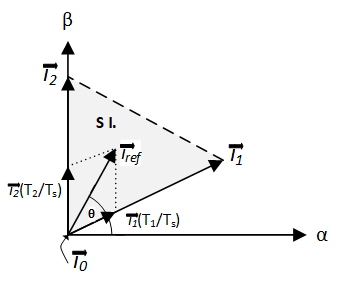
\includegraphics[width=0.6\textwidth]{EMPC_PNG_Pics/OnePhasor.png}
        \caption{Synthesis of $\protect\overrightarrow{i_{ref}}$ by $\protect\overrightarrow{i_{1}}$, $\protect\overrightarrow{i_{2}}$, and $\protect\overrightarrow{i_{0}}$}
        \label{EMPC:fig:OnePhasor}
    \end{figure}

    The complex plane is naturally divided by the fundamental space vectors into six areas, named "sectors".

    \begin{equation}
        \begin{array}{l}
            x\frac{\pi}{6}+\frac{(n-1)\pi}{3}\leq\theta_n\leq\frac{\pi}{6}+\frac{n\pi}{3}\\
            n=1,2,\dots,6
        \end{array}
        \label{EMPC:equ:angle}
    \end{equation}

    The non-zero space vectors are selected based on the phase angle $\theta$ between $\overrightarrow{i_{ref}}$ and the real axis.
    Table \ref{EMPC:tbl:sequence} presents an example of switching pattern in case of a current reference vector situated in Sector I.

    \begin{table}[]

		\caption{Representation of switching sequences for SECTOR I.}
		\centering
        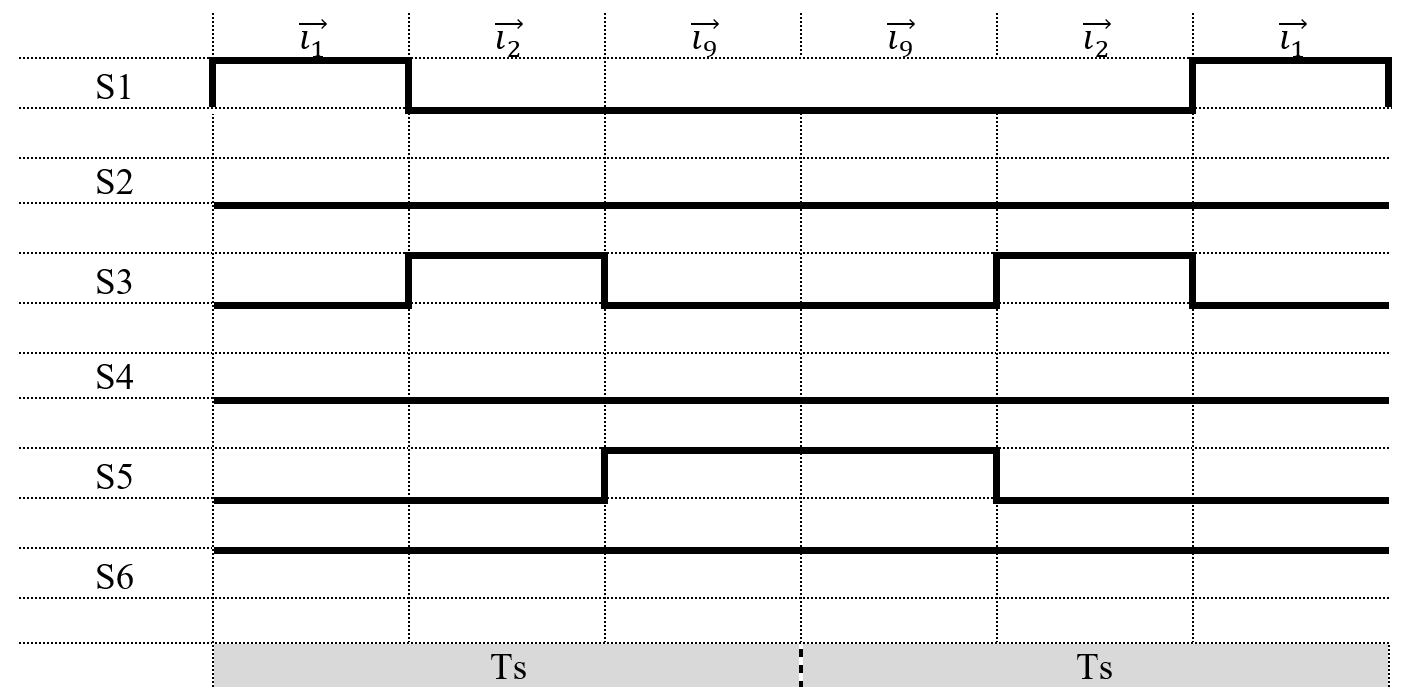
\includegraphics[width=0.8\textwidth]{EMPC_PNG_Pics/Sequence.png}

        \label{EMPC:tbl:sequence}
    \end{table}

    The switching scheme represented in Table \ref{EMPC:tbl:fundamental_vect}. is aimed at reducing the number of commutations in a switching cycle, resulting in the reduction of the switching losses \cite{moussaoui2005open}.
    Additionally, the constraint (\ref{EMPC:equ:refconstraint}) resulting from the available magnitudes of the current vectors, is applied to the current reference.

    \begin{equation}
        \begin{array}{l}
            0\leq|i_{ref}|\leq\frac{\sqrt{6}i_{dc}}{cos\theta+\sqrt{3}sin\theta}
        \end{array}
        \label{EMPC:equ:refconstraint}
    \end{equation}

\subsection{Discussion}\label{EMPC:sec:Discussion}

    From the continuous AC \ref{EMPC:equ:mtx_AC}, and DC \ref{EMPC:equ:mtx_DC} model equations described in Ch.X., the controller is formulated form discretised system \ref{EMPC:equ:DiscreteStateSpace}, and it is described via the cost function and control problem of \ref{EMPC:equ:optim_problem}, and \ref{EMPC:equ:optim_problem_constr} in Ch.X$+$1. The evaluated model and control structure are shown on Fig.4. In the following section said EMPC’s computational requirements are evaluated, and the Matlab/Simulink simulation results are compared to a classic state feedback controller’s dynamic performance.

    \subsubsection{Computational effort}\label{EMPC:sec:CompEffort}

    The binary search tree generated for the control problem presented in Fig. \ref{EMPC:fig:SearchTree}. The search method and formulation of the tree is described in chapter \ref{BASICCSR:sec:EMPCStorage}. The depth of the search tree is 5 and it has a total number of 29 nodes. It is utilized with the MPT toolbox \cite{muthukumar2016adaptive}, \cite{kutasi2010constrained}, and it can be used for the computationally optimal real-time implementation of the proposed algorithm on low-cost hardware.

    \begin{figure}[!ht]
        \centering
        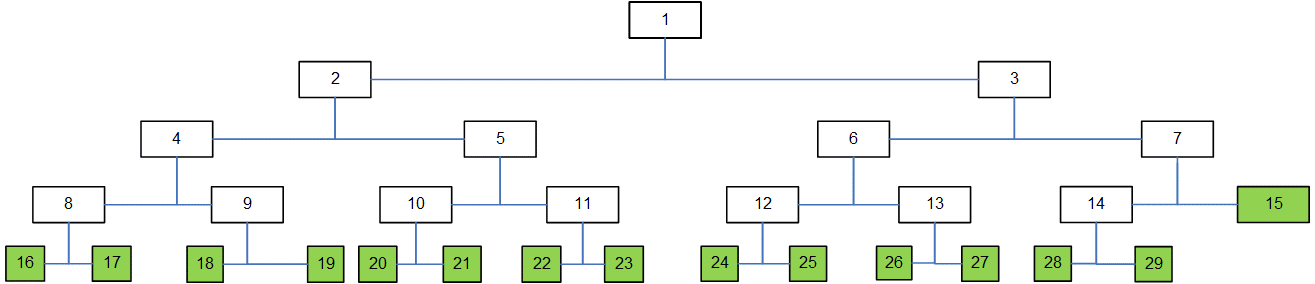
\includegraphics[width=\textwidth]{EMPC_PNG_Pics/SearchTree.png}
        \caption{Binary search tree of the controller for a horizon of $N = 4$. The leaf nodes are depicted with filled squares. The depth of the tree is 5.}
        \label{EMPC:fig:SearchTree}
    \end{figure}

    The search for an active critical region starts from the first level and represents the evaluation in each adjacent node of an inequality of the form: $x\leq K$. Thus, in this case a maximum number of 4 inequalities have to be evaluated to reach the active critical region. Implementing the presented algorithm is straightforward on a DSP processor, for instance from the dsPIC33 family by Microchip. Using the MAC (multiply and accumulate) instruction the inequality is evaluated for each node using 4 instructions, thus in 80 ns on a 50 MIPS processor (Fig. \ref{EMPC:fig:Memory}). The active critical region can be reached in a maximum of 400 ns. Compared to the typical sample rate of 10us in the case of a CSR, the real-time implementation on a DSP processor is possible. More information about storing critical regions can be found in \oldref{BASICCSR:sec:EMPCStorage}.
    
    \begin{figure}[!ht]
        \centering
        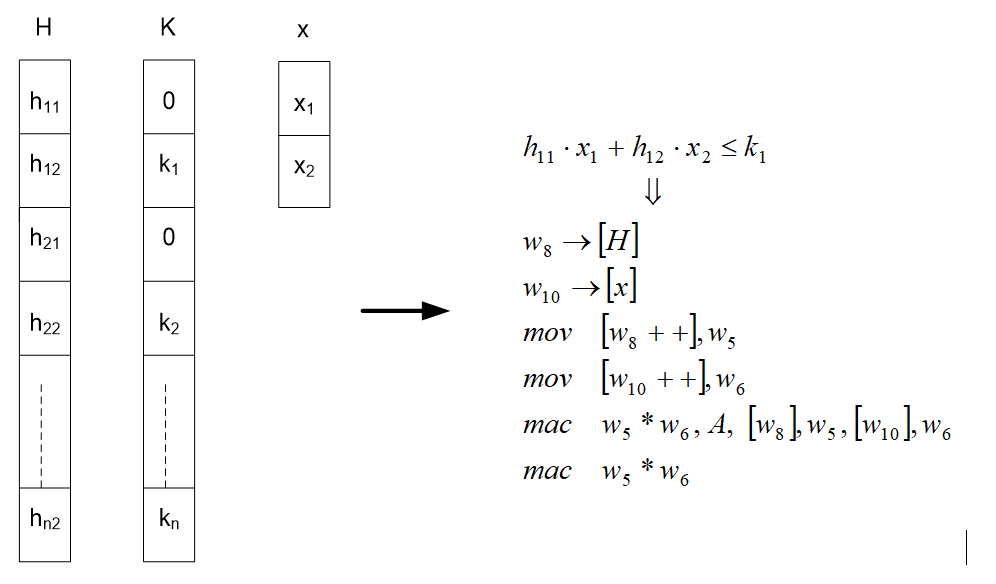
\includegraphics[width=\textwidth]{EMPC_PNG_Pics/Memory.png}
        \caption{Data organization in the data memory of a single core DSP and the evaluation of a 2-dimensional inequality}
        \label{EMPC:fig:Memory}
    \end{figure}
    
    More information about storing critical regions can be found in \oldref{BASICCSR:sec:EMPCStorage}.

    \subsubsection{Horizon performance}\label{EMPC:sec:Performance}

    With the cost function (\ref{EMPC:equ:optim_problem}) employed using (\ref{EMPC:equ:quadratic_mtx_set}), changing the length of the horizon ($N$) affects the system's complexity illustrated by the partition in the state space shown in Fig. \ref{EMPC:fig:regions}., and Fig. \ref{EMPC:fig:MultiHorizon} presents the step response of the controlled system for different lengths of the horizon. It shows, that the response is not affected by the increase of the horizon above $N=2$, supporting the choice of this value for Matlab Simulink implementation.

    \begin{figure}[!ht]
        \centering
        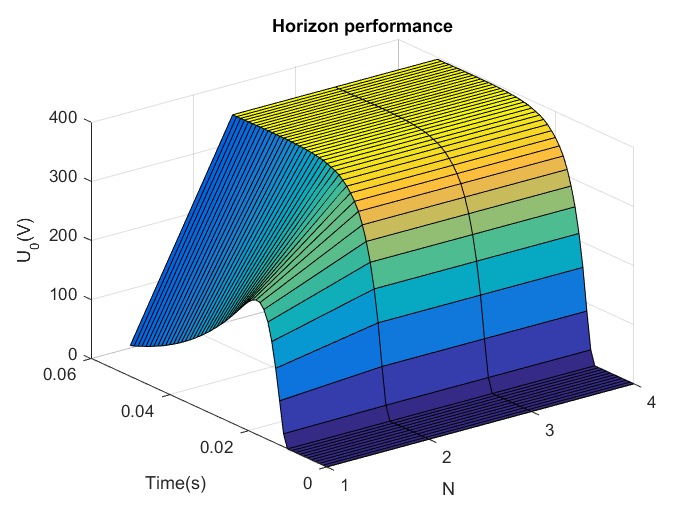
\includegraphics[width=\textwidth]{EMPC_PNG_Pics/MultiHorizon.png}
        \caption{Step response of the system as a function of the horizon length (N).}
        \label{EMPC:fig:MultiHorizon}
    \end{figure}

    \subsubsection{Simulation results}\label{EMPC:sec:Results}

    The simulation results are produced with Matlab/Simulik. The discrete model's (\ref{EMPC:equ:DiscreteStateSpace}) simulation frequency was 1 MHz, with the model parameters represented in Table \ref{EMPC:tbl:params}., and with the control structure shown on Fig. \ref{EMPC:fig:ControlStruct}. The EMPC performance is shown below:

    \begin{figure}[!ht]
        \centering
        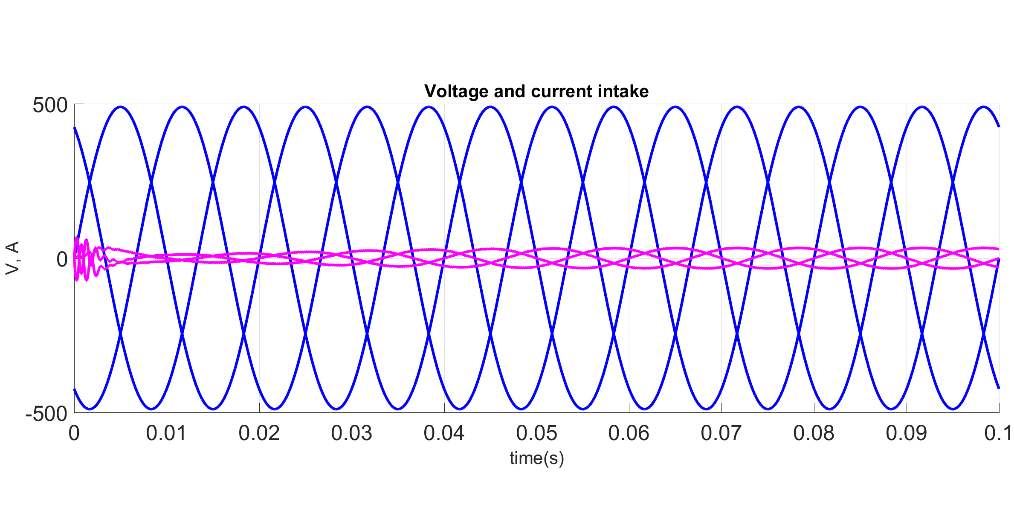
\includegraphics[width=\textwidth]{EMPC_PNG_Pics/Result_3fEMPC.png}
        \caption{Three-phase voltage and current intake of the CSR with EMPC}
        \label{EMPC:fig:Result_3fEMPC}
    \end{figure}

    \begin{figure}[!ht]
        \centering
        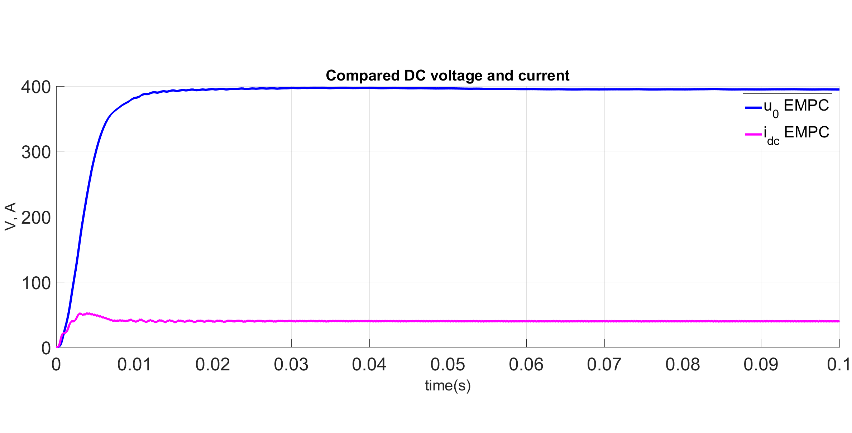
\includegraphics[width=\textwidth]{EMPC_PNG_Pics/Result_PerformanceEMPC.png}
        \caption{Resulting current and voltage trajectories of the CSR with (EMPC).}
        \label{EMPC:fig:Result_PerformanceEMPC}
    \end{figure}

    More details about the Matlab simulation are presented in \cite{neukirchner2019linkedmodel}.

    \subsubsection{Comparison with a state feedback control}\label{EMPC:sec:Comparison}

    On the DC side, not only the output voltage $u_0$ but also the inductor current $i_{dc}$ needs to be controlled. Described in [28], a state feedback control with optimal parameters can be used as a reference based on the model properties listed in Table \ref{EMPC:tbl:params}, with output voltage $u_0$ and DC bus current $i_{dc}$ chosen as the state variables. Since $u_0$ is a DC quantity in steady state, an integrator signal is introduced to diminish the steady-state error. The structure of the controller is represented in Fig. \ref{EMPC:fig:SFeedbackDC}.

    \begin{figure}[!ht]
        \centering
        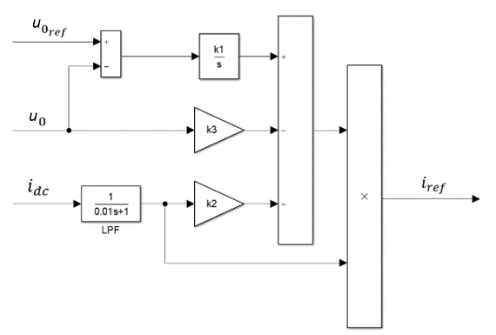
\includegraphics[width=0.7\textwidth]{EMPC_PNG_Pics/SFeedbackDC.png}
        \caption{Simple DC side state feedback control structure.}
        \label{EMPC:fig:SFeedbackDC}
    \end{figure}

    The tuning constants applied and calculated according to \cite{godlewska2015predictive} are:

    \begin{equation}
        \begin{array}{l}
            k1=\frac{\omega^3_n}{1.5U_n\omega^2_{dc}},\,k2=\frac{1.9\omega_n L_{dc}}{1.5U_n},\,k3=\frac{2.2\omega^2_n}{1.5U_n(\omega^2_{dc}-1)},\\
            \textnormal{where,}\\
            \omega_n=1.1,\,\omega_{ac}=\frac{1}{\sqrt{L_{ac}C_{ac}}},\,\omega_{dc}=\frac{1}{\sqrt{L_{dc}C_{dc}}}
        \end{array}
        \label{EMPC:equ:tuning}
    \end{equation}

    The state feedback controllers block on the diagram is taking the controller's place, shown on Fig. \ref{EMPC:fig:ControlStruct}. The independent outputs are the high pass filter's output  $i_{rHPF(d)}$ and the controller's output $i_{rcontrol(d)}$. The sum of the independent current values is converted to Clarke frame to be able to govern the switching states of the IGBT's. This can be done because $i_{rHF(d)}$ has only high frequency components and $i_{rcontrol(d)}$ has low frequency components due to the differences in LC time constants, as discussed in the second section. Then the control signal governing the switches is applied in the same manner, described at the start of section \oldref{EMPC:sec:Modulation}.
    The state feedback control's performance in comparison with the EMPC is shown in Fig. \ref{EMPC:fig:Result_EMPCfinal}.

    \begin{figure}[!ht]
        \centering
        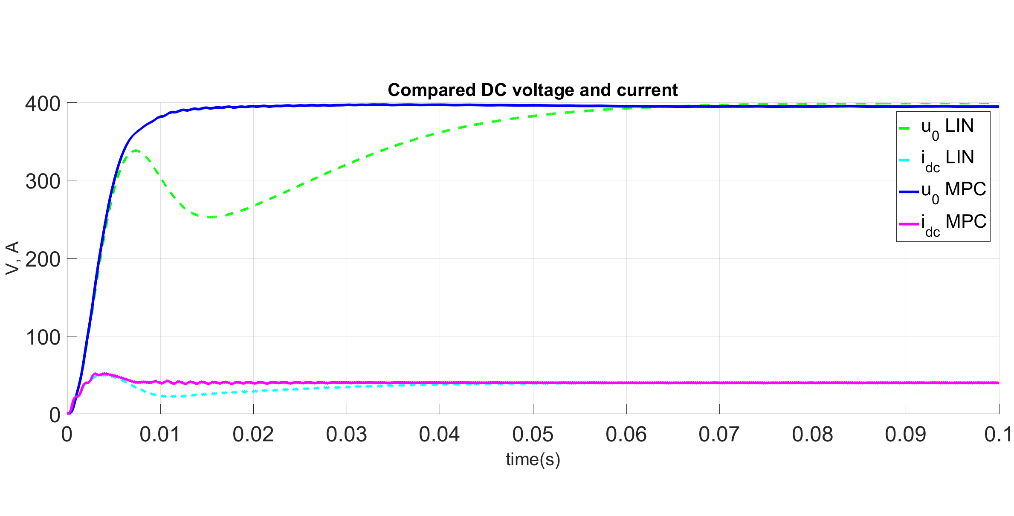
\includegraphics[width=\textwidth]{EMPC_PNG_Pics/Result_EMPCfinal.png}
        \caption{Resulting current and voltage trajectories of the CSR with explicit model predictive control (MPC) compared state feedback control (LIN).}
        \label{EMPC:fig:Result_EMPCfinal}
    \end{figure}

\section{Conclusion}\label{EMPC:sec:Conclusions}

    The constrained, model-based optimal control of a current source rectifier has been presented in this dissertation. The dynamic model of a three-phase current source rectifier has been developed in Park frame. The proposed model has been examined from the design and implementation points of view with the purpose of explicit model-based predictive control. It proved to be the case that the regular set of differential equations of the CSR appears to be too complex, and contains non-linearity for such a design approach. To address this issue the usage of separated AC and DC equation sets was suggested to avoid linearization and complexity reduction. This solution eliminates bilinearity and enables the application of linear control design techniques. Current-based SVPWM of the three-phase converter has been used with an emphasis on the reduction of switching losses. Throughout the chapter the explicit model predictive control method is described and the method's effectiveness compared to conventional state feedback control is show. The implementation and simulation experiments have been performed in Matlab/Simulink environment. Moreover, the proper implementation of the system in a modern DSP chip will result in real-time operation. 